\documentclass[
	ngerman,
	%twoside,
	BCOR=8mm,
	headings=normal,
	parskip=half,
	headsepline,
	automark,
	listof=totoc,
	bibliography=totoc,
	%,captions=tableabove
	%draft
]{scrreprt}
\usepackage{graphicx}
%
%
%%%%%%%%%%%%%%%%%%%%%%%%%%%%%%%%%%%%%%%%%%%%%%%%%%%%%%%%%%%%%%%%%%%%%%%%%%%%%%%
% Pakete laden
%%%%%%%%%%%%%%%%%%%%%%%%%%%%%%%%%%%%%%%%%%%%%%%%%%%%%%%%%%%%%%%%%%%%%%%%%%%%%%%
%
\usepackage{ifluatex}
\usepackage{babel}
%
\ifluatex
 % LuaLaTeX
 \usepackage{fontspec}
 \usepackage{selnolig}
\else
 % PdfLaTeX
 \usepackage[T1]{fontenc}
\fi
%
\usepackage{csquotes}
\usepackage{scrlayer-scrpage}
\usepackage{microtype}
%
%\usepackage{ziffer}% optional
%\usepackage[locale=DE]{siunitx}% optional
%
\usepackage{tikz}
\usepackage{pgfplots}
%
\usepackage[style=ieee,backend=biber,language=german]{biblatex}
%
\usepackage{amsmath}
\usepackage{amssymb}
\usepackage{epigraph}
\usepackage{courier}
\usepackage{longtable}
\usepackage{array}
\usepackage{svg}
\usepackage{float}
%
% compile fix
\usepackage{lmodern}

\usepackage{hyperref}
%
%=== wichtig, dass folgende Pakete NACH hyperref geladen werden ===============
\usepackage{scrhack}% Um Warnung bzgl. \float@addtolists im listings-Paket (s.u.) zu vermeiden
\usepackage{listings}
%
\usepackage[nameinlink]{cleveref}
\usepackage[all]{hypcap}
\usepackage[
	toc,
	symbols,
	acronyms,
]{glossaries}
%
%%%%%%%%%%%%%%%%%%%%%%%%%%%%%%%%%%%%%%%%%%%%%%%%%%%%%%%%%%%%%%%%%%%%%%%%%%%%%%%
% Globale Definitionen
%%%%%%%%%%%%%%%%%%%%%%%%%%%%%%%%%%%%%%%%%%%%%%%%%%%%%%%%%%%%%%%%%%%%%%%%%%%%%%%

%=== pdf Metadaten ============================================================
\hypersetup{
	pdfauthor={Vorname Nachname},
	pdftitle={Vorlage für wissenschaftliche Abschlussarbeiten an der TH Köln},
	pdfsubject={Abschlussarbeit},
	pdfkeywords={
		LaTeX,
		Abschlussarbeit,
		Vorlage,
	},
	bookmarksnumbered=true,
	pdfstartview=FitH,
	hidelinks,
}

%=== Vorwort vor Literatur ====================================================
\defbibnote{mynote}{%
	Wie in \cref{sec:bib-content} erläutert, werden im Literaturverzeichnis 
	ausschließlich die Quellen angegeben, auf die im Rahmen einer Arbeit 
	tatsächlich verwiesen wird. Bitte prüfen Sie also das Literaturverzeichnis 
	Ihrer Arbeit immer dahingehend, ob alle zitierten Quellen~--~und nur
	diese~--~erfasst wurden. Dies trifft auf das nun folgende Verzeichnis
	\emph{nicht} zu; die 
	meisten der hier aufgeführten Quellen werden in dieser Vorlage nicht 
	zitiert. Es handelt sich lediglich um ein Beispiel für ein 
	Literaturverzeichnis mit Literaturempfehlungen zum wissenschaftlichen 
	Schreiben.
}

%=== Kopf-/Fusszeile definieren ===============================================
\clearpairofpagestyles
\ohead[]{\headmark}
\ofoot[\pagemark]{\pagemark}

%=== Farben definieren ========================================================
\definecolor{THRed}{RGB}{207,24,32}
\definecolor{THOrange}{RGB}{236,101,37}
\definecolor{THPurple}{RGB}{175,54,140}

%=== Einstellungen für cref ===================================================
\newcommand{\crefpairconjunction}{ und~}
\newcommand{\crefrangeconjunction}{ bis~}
\crefname{figure}{Abbildung}{Abbildungen}

%=== Einstellungen für plots ==================================================
\pgfplotsset{
	compat=newest,
	/pgf/number format/.cd,
	dec sep={\text{,}},
	1000 sep={\,},
}

%=== Einstellungen für listings ===============================================
\lstdefinestyle{myLaTeX}{
	basicstyle=\footnotesize\ttfamily,
	language=TeX,
	keywordstyle=\color{blue},
	frame=single,
	backgroundcolor=\color{gray!10},
	tabsize=2,
	morekeywords={
		lstdefinestyle,
		footnotesize,
		ttfamily,
		color,
	},
}

\lstdefinestyle{myBasic}{
	basicstyle=\footnotesize\ttfamily,
	frame=single,
	escapechar={|_},
	backgroundcolor=\color{white},
	keywordstyle=\color{black},
}

\lstset{style=myLaTeX}

%\lstset{language=Python, basicstyle=\small, frame=single, numbers=left, xleftmargin=2em, framexleftmargin=1.5em}
%\renewcommand{\lstlistingname}{Algorithmus}


%=== paar convenience Sachen definieren =======================================
\DeclareMathOperator{\sgn}{sgn}
\newcommand{\vecW}{\ensuremath{\mathbf{w}}}%
\newcommand{\ci}{\ensuremath{\mathrm{i}}}%
%
\newcommand{\tb}{\textbackslash}
%
\newcommand{\comm}[1]{\enquote{\texttt{\tb #1}}}
%
\newcommand{\param}[1]{%
	$\langle$\textrm{\textit{#1}}$\rangle$%
}

%=== Arial als Hauptschriftart ================================================
%\setsansfont{Arial}
%\renewcommand{\familydefault}{\sfdefault}

%
%%%%%%%%%%%%%%%%%%%%%%%%%%%%%%%%%%%%%%%%%%%%%%%%%%%%%%%%%%%%%%%%%%%%%%%%%%%%%%%
% Begriffe für glossaries definieren
%%%%%%%%%%%%%%%%%%%%%%%%%%%%%%%%%%%%%%%%%%%%%%%%%%%%%%%%%%%%%%%%%%%%%%%%%%%%%%%

%=== Glossar ==================================================================
\newglossaryentry{plugin}{
	name={Plugin},
	description={Softwareerweiterung bestehend aus Codepaketen, die die
	Kernfunktionalität von WordPress erweitern. Plugins bestehen
	aus PHP-Code und können weitere Assets wie Bilder, CSS und
	JavaScript enthalten. \\(eigene Übersetzung nach \cite{wordpress2024plugin})}
}
\newglossaryentry{wdr}{
	name={Wordpress Developer Resources},
	description={Ein online Handbuch, das Entwicklungsthemen in Wordpress abdeckt. Es wird kontinuierlich weiterentwickelt und gibt Entwicklern Definitionen, Coding Standards, Wordpress Core Ressources, Block Editor Ressources, gängige APIs, Beispiele und Tutorials an die Hand}
}
\newglossaryentry{csr}{
    name={Corporate Social Responsibility},
    description={Unter "Corporate Social Responsibility" (CSR) ist die gesellschaftliche Verantwortung von Unternehmen im Sinne eines nachhaltigen Wirtschaftens zu verstehen.\cite{BMAS2022_CSRGrundlagen}}
}
\newglossaryentry{dog}{
	name={Hund},
	description={Behaartes, vierbeiniges Säugetier. Bester Freund des
	Menschen}
}

%=== Abkürzungen ==============================================================
\newacronym{svm}{SVM}{support vector machine}

\newacronym{acf}{ACF PRO}{Advanced Custom Fields Pro}
\newacronym{ajax}{AJAX}{Asynchronous JavaScript and XML}
\newacronym{api}{API}{Application Programming Interface}
\newacronym{b2b}{B2B}{Business-to-Business}
\newacronym{b2c}{B2C}{Business-to-Consumer}
\newacronym{cdn}{CDN}{Content Delivery Network}
\newacronym{ci}{CI}{Corporate Identity}
\newacronym{cli}{CLI}{Command Line Interface}
\newacronym{cms}{CMS}{Content-Management-System}
\newacronym{crm}{CRM}{Customer-Relationship-Management}
\newacronym{csr}{CSR}{Corporate Social Responsibility}
\newacronym{csrf}{CSRF}{Cross-Site Request Forgery}
\newacronym{css}{CSS}{Cascading Style Sheets}
\newacronym{cta}{CTA}{Call to Action}
\newacronym{gnu}{GNU}{GNU's Not Unix}
\newacronym{gpl}{GPL}{General Public License}
\newacronym{gsap}{GSAP}{GreenSock Animation Platform}
\newacronym{http}{HTTP}{Hypertext Transfer Protocol}
\newacronym{js}{JS}{JavaScript}
\newacronym{json}{JSON}{JavaScript Object Notation}
\newacronym{kpi}{KPI}{Key Performance Indicator}
\newacronym{mp4}{MP4}{Moving Picture Experts Group 4 Part 14}
\newacronym{mysql}{MySQL}{My Structured Query Language}
\newacronym{npm}{NPM}{Node Package Manager}
\newacronym{orm}{ORM}{Object-Relational Mapping}
\newacronym{php}{PHP}{Hypertext Preprocessor}
\newacronym{rest}{REST}{Representational State Transfer}
\newacronym{smtp}{SMTP}{Simple Mail Transfer Protocol}
\newacronym{ssl}{SSL}{Secure Sockets Layer}
\newacronym{sql}{SQL}{Structured Query Language}
\newacronym{tls}{TLS}{Transport Layer Security}
\newacronym{uri}{URI}{Uniform Resource Identifier}
\newacronym{url}{URL}{Uniform Resource Locator}
\newacronym{wp}{WP}{WordPress}
\newacronym{xml}{XML}{Extensible Markup Language}
\newacronym{xsl}{XSL}{Extensible Stylesheet Language}
\newacronym{xss}{XSS}{Cross-Site-Scripting}

%=== Symbole ==================================================================
\newglossaryentry{sym:force}{
	name=\ensuremath{\vec{F}},
	description={Kraft, vektorielle Größe},
	type=symbols,
}

%
\makeglossaries
%
\graphicspath{{images/}}
%
\addbibresource{references.bib}

\nocite{*} % listet alle Quellen (auch die nicht zitierten!)
%
%=== für schnelleres kopilieren alle ungeänderten Dateien auskommentieren =====
\includeonly{
    content/chapDeclaration,
    content/chapAbstract,
    content/chapEinleitung,
	content/chapBasics,
    content/chapContext,
    content/chapConceptDesign,
    content/chapImplement
}
%
%
%==============================================================================
%
\begin{document}
%
\pdfbookmark[0]{Titelseite}{titel}
\begin{titlepage}
%
\sffamily% Umschalten auf serifenlose Schrift
%
\begin{center}
\begin{tikzpicture}
 \fill[THRed] (0, 0) rectangle (\textwidth/3, 3pt);
 \fill[THOrange] (\textwidth/3, 0) rectangle (2*\textwidth/3, 3pt);
 \fill[THPurple] (2*\textwidth/3, 0) rectangle (\textwidth, 3pt);
\end{tikzpicture}
\end{center}
%
\vfill
%
\begin{huge}
    Weiterentwicklung eines WordPress-Plugins zur gamifizierten Spendenverteilung:
    Gutenberg-Integration und Plugin-Architektur am Beispiel von ``Charigame'' in Kooperation mit der elancer-team GmbH\\[10mm]
\end{huge}
%
Bachelorarbeit zur Erlangung des akademischen Grades\newline
\emph{Bachelor of Science}\newline
im Studiengang Medieninformatik\newline
an der Fakultät für Informatik und Ingenieurwissenschaften\newline
der Technischen Hochschule Köln
%
\vfill
%
\begin{tabular}{@{}ll}
vorgelegt von: & Christian Krenn\\
               & chrsitian.krenn@smail.th-koeln.de\\[5mm]
eingereicht bei:   & Prof. Dr. Hoai Viet Nguyen\\
Zweitgutachter*in: & Tobias Derksen
\end{tabular}	
%
\\[10mm]
%
Gummersbach, 03.09.2025%
%
\rmfamily% Umschalten auf Standard-Schrift mit Serifen
%
\end{titlepage}
\cleardoublepage
\pagenumbering{Roman}
\chapter*{Kurzfassung/\emph{Abstract}}
\label{chap:abstract}
%


\cleardoublepage
\pdfbookmark[0]{Inhaltsverzeichnis}{toc}
\tableofcontents
\listoftables
\listoffigures
\printglossary
\printglossary[type=\acronymtype, title={Abkürzungsverzeichnis}]
\printglossary[type=symbols, title={Symbolverzeichnis}]
%
\cleardoublepage
\KOMAoptions{open=right}
\pagenumbering{arabic}
\chapter{Einleitung}
\begin{quote}
    ``Simplicity is a great virtue but it requires hard work to achieve it and education to appreciate it. And to make matters worse: complexity sells better.''
\end{quote}
\cite{dijkstra1982}

\section{Problemstellung und Motivation}
\section{Zielsetzung der Arbeit}
\section{Aufbau der Arbeit}
%
Das vorliegende Dokument kann als Muster und Anleitung für wissenschaftliche Abschlussarbeiten verwendet werden. Es beruht ursprünglich auf einem Leitfaden, den Prof.~Dr.~Stephan Freichel als Prüfungsausschussvorsitzender für die Studiengänge B.\,Sc.~Logistik und M.\,Sc.~\emph{Supply Chain and Operations Management} an der Fakultät für Fahrzeugsysteme und Produktion erstellt hat.
\par
Der Text in dieser Vorlage beschreibt allgemeine formale Anforderungen, insbesondere zum Inhaltsverzeichnis, zum Einfügen von Quellenverweisen und zum Erstellen eines Literaturverzeichnisses.
\par
Die Vorlage kann fachübergreifend als Musterdatei für Abschlussarbeiten an der TH Köln verwendet werden. Allerdings müssen Sie dann unbedingt klären, ob sie den Konventionen in ihrem Studienfach entspricht.
\par
Für die Möglichkeit eines fachunabhängigen Gebrauchs wurde das Dokument von Maria-Anna Worth (i.\,R.) und Susanne Neuzerling (Hochschulreferat Planung und Controlling) inhaltlich überarbeitet und modifiziert. Eine erneute Überarbeitung und Aktualisierung erfolgte durch Andreas Bissels (Schreibzentrum). Frau Katharina Bata hat die Dokumentvorlage in LaTeX erstellt. Zuletzt wurde diese Vorlage 2023 von André Ulrich und Jan Salmen überarbeitet und um diverse Hinweise speziell zur Gestaltung mit \LaTeX{} ergänzt (siehe \cref{chap:Textsatz}).
\par
Zur Vorbereitung auf Ihre Abschlussarbeit empfehlen wir Ihnen die Angebote des Schreibzentrums der Kompetenzwerkstatt\footnote{\href{https://www.th-koeln.de/schreibzentrum}{https://www.th-koeln.de/schreibzentrum}}; hierzu gehören sowohl eine Schreibberatung als auch Schreibkurse. Das Schreibzentrum ist Ihre Anlaufstelle an der TH Köln in Fragen rund um das wissenschaftliche Schreiben.
\par
Sichern Sie diese Dokumentvorlage bitte zweifach auf Ihrem Rechner: Einmal, um weiterhin auf den hier dargestellten Inhalt zugreifen zu können, und ein zweites Mal, um sie mit Ihrer eigenen Abschlussarbeit zu überschreiben.
\par
\emph{Bitte beachten Sie: Die Vorlage ersetzt nicht die spezifischen Vorgaben der jeweiligen Prüfungsausschüsse. Sollte es in Ihrem Fach besondere formale Vorgaben geben, so gelten diese.}\enlargethispage{\baselineskip}
%
\begin{flushright}
Köln, August 2023
\end{flushright}
\chapter{Theoretische Grundlagen}
\section{WordPress als Content-Management-System}
\section{Plugin-Entwicklung mit WordPress}
\section{Gutenberg-Editor: Konzept und technische Grundlagen}
\section{Gamification im Kontext digitaler Anwendungen}
\section{Überblick über Spendenverteilung und Charity-Plattformen}
\label{chap:formal}
%
In diesem Kapitel finden Sie grundlegende Hinweise zum formalen Aufbau Ihrer Arbeit.
%
\textbf{Reihenfolge}
\label{sec:aufbau}
Eine wissenschaftliche Arbeit besteht in der Regel aus den folgenden Teilen:
%
\begin{enumerate}
 \item Deckblatt
 \item Kurzfassung/Abstract (optional)
 \item Inhaltsverzeichnis
 \item Abbildungs- und Tabellenverzeichnis (auch am Ende üblich)
 \item Abkürzungsverzeichnis (auch am Ende üblich)
 \item Einleitung
 \item Hauptteil
 \item Zusammenfassung/Fazit
 \item Literaturverzeichnis
 \item Anhänge (optional)
 \item Erklärung
\end{enumerate}
%
%
\textbf{Deckblatt}
%Die Gestaltung des Deckblatts folgt den visuellen Vorgaben für Publikationen der TH Köln.
%\par
Das Deckblatt beinhaltet: Titel der Arbeit, Art der Arbeit, Verfasser*in, Matrikelnummer, Abgabetermin, Betreuer*in sowie Zweitgutachter*in. Das Deckblatt wird bei Arbeiten, die länger sind als~15 Seiten, bei der Seitenanzahl zwar mitgezählt, jedoch nicht nummeriert.
%
%
\textbf{Inhaltsverzeichnis}
\label{sec:listOfContents}
Wir empfehlen eine Dezimalgliederung wie in diesem Dokument angelegt. Werden innerhalb eines Kapitels Unterüberschriften verwendet, müssen mindestens zwei vorhanden sein: wo ein~2.1 ist, muss es ein~2.2 geben.
\par
Das Inhaltsverzeichnis enthält immer die Seitenangaben zu den aufgelisteten Gliederungspunkten; es wird dabei aber selbst nicht im Inhaltsverzeichnis aufgelistet. Die Seiten, die das Inhaltsverzeichnis selbst einnimmt, können römisch gezählt werden.
%Mehr hierzu in Abschnitt~\cref{}.
\par
Für eine Abschlussarbeit ist eine Gliederungstiefe von wenigstens drei Ebenen üblich. In der Regel werden nur bis zu vier Ebenen vorne im Inhaltsverzeichnis abgebildet. Hier sollten Sie aber unbedingt die Gepflogenheiten in Ihrem Fach berücksichtigen und ggf. in Erfahrung bringen.
%\par
%In dieser Word-Vorlage wird das Inhaltsverzeichnis für die Überschriftenebenen 1 bis 3 automatisch generiert (Rechtsklick auf das Inhaltsverzeichnis > Felder aktualisieren > Ganzes Verzeichnis).
%
%
\textbf{Abbildungsverzeichnis und Tabellenverzeichnis}
Abbildungen und Tabellen werden in entsprechenden Verzeichnissen gelistet. In dieser Vorlage erscheinen sie direkt nach dem Inhaltsverzeichnis. Dann können die entsprechenden Seiten römisch gezählt werden. Die Verzeichnisse können jedoch auch am Ende der Arbeit vor oder hinter dem Literaturverzeichnis stehen. Dann werden sie regulär mit Seitenzahlen versehen.
%Verzeichnisüberschriften (z. B. Abbildungsverzeichnis) werden nie nummeriert (Formatvorlage Überschrift 1 unnummeriert verwenden).
%
%
\textbf{Abkürzungsverzeichnis}
Die Zahl der Abkürzungen sollte übersichtlich bleiben. Das Abkürzungsverzeichnis enthält lediglich wichtige fachspezifischen Abkürzungen in alphabetischer Reihenfolge, insbesondere Abkürzungen von Organisationen, Verbänden oder Gesetzen. Gängige Abkürzungen wie \enquote{u.\,a.}, \enquote{z.\,B.}, \enquote{etc.} werden nicht aufgenommen.
\par
Zur technischen Umsetzung mit \LaTeX{} vergleiche auch Abschnitt~\ref{sec:template}.
%
%
\textbf{Literaturverzeichnis}
Das Literaturverzeichnis wird alphabetisch nach Autorennamen geordnet. Es enthält alle im Text zitierten Quellen~--~und nur diese. Mehrere Schriften einer Person werden nach Erscheinungsjahr geordnet. Schriften derselben Person aus einem Erscheinungsjahr müssen Sie selbst unterscheidbar machen. In den Ingenieurwissenschaften wird zusätzlich häufig ein Nummern- oder Autorenkürzel dem Namen in eckigen Klammern voran-gestellt. Mehr hierzu und weitere wichtige Regeln des Zitierens lernen Sie in den E-Learning-Kursen des Schreibzentrums\footnote{\href{https://ilu.th-koeln.de/goto.php?target=cat\_52109\&client\_id=thkilu}{https://ilu.th-koeln.de/goto.php?target=cat\_52109\&client\_id=thkilu}} kennen.
\par
Zur Verwaltung der verwendeten Literatur eigenen sich entsprechende Softwaretools wie Citavi oder Zotero, die mit verschiedenen Textverarbeitungsprogrammen kompatibel sind.
%
%
\textbf{Rechtschreibung, Grammatik}
Achten Sie bei der Abgabe Ihrer Arbeit auf ein einwandfreies Deutsch bzw. Englisch. Wenn Fehler die Lesbarkeit beeinträchtigen, kann sich dies durchaus negativ auf die Note auswirken. Nutzen Sie daher unbedingt die Rechtschreibprüfung Ihres Textverarbeitungsprogramms, auch wenn diese nicht alle Fehler erkennt.
%In Word können Sie diese unter Datei > Optionen > Dokumentenprüfung bearbeiten sowie ein- und ausschalten.
\par
Für alle, die sich bei diesem Thema unsicher fühlen, empfehlen wir die E-Learning-Kurse des Schreibzentrums\footnote{\href{https://ilu.th-koeln.de/goto.php?target=cat\_52109\&client\_id=thkilu}{https://ilu.th-koeln.de/goto.php?target=cat\_52109\&client\_id=thkilu}}. Wenden Sie sich ggf. auch an die Beauftragte für Studierende mit Beeinträchtigung\footnote{\href{https://www.th-koeln.de/studium/studieren-mit-beeintraechtigung\_169.php}{https://www.th-koeln.de/studium/studieren-mit-beeintraechtigung\_169.php}}.
%
%
\textbf{Umfang der Arbeit}
Alle Fächer nennen verbindliche Angaben zu Unter- und Obergrenzen, die in der Regel eingehalten werden müssen. Verzeichnisse und Anhänge werden dabei in aller Regel nicht mitgezählt. In Einzelfällen~--~insbesondere bei empirischen Arbeiten~--~können abweichende Vereinbarungen mit der Betreuungsperson getroffen werden.
\chapter{Projektkontext}
\label{chap:Textsatz}
%
Mit \LaTeX{} ist es verhältnismäßig einfach, Dokumente zu erstellen, die professionellen Ansprüchen genügen. Ein entscheidender Vorteil ist, dass der Nutzer fast nur den Inhalt beisteuert, während die korrekte äußere Form dann automatisch erzeugt wird. \LaTeX{} basiert auf \TeX{}, das von Donald Knuth entwickelt wurde~\cite{knuth:tex}. Einige weitere Vorteile gegenüber gängiger
Textverarbeitung:
\begin{description}
	\item[Frei/Plattformunabhägig:] Bei \LaTeX{} handelt es sich um freie 
	Software. Es wird kein proprietärer Editor benötigt, um \LaTeX{}-Dokumente
	zu schreiben. Tatsächlich können die Dokumente auf \emph{jedem} Rechner
	mit \emph{jedem} beliebigen Editor bearbeitet werden.
	%
	\item[Reines Textformat:] Der Quelltext~--~die \texttt{tex}-Datei~--~ist
	ein reines Textformat. Dadurch eignen sich \LaTeX{}-Dokumente auch 
	hervorragend zur Versionskontrolle mit beispielsweise git. Dies wiederum
	ermöglicht eine effiziente Zusammenarbeit mehrerer Autor*innen.
	%
	\item[Aufteilen großer Dokumente:] Der Quelltext großer Dokumente, wie 
	beispielsweise von Projektarbeiten, kann auf mehrere Dateien
	aufgeteilt werden. So können beispielsweise mehrere Personen an jeweils
	einem eigenen Kapitel arbeiten. Aufgrund der beiden oberen Punkte wird es 
	auch nicht zu Kompatibilitätsproblemen kommen.
	%
	\item[Trennen von Layout/Inhalt:] Mit \LaTeX{} kann man explizit das
	Layout für das gesamte Dokument festlegen -- oder die verwendete 
	Dokumentklasse kümmert sich implizit darum. Zeitgemäße Textverarbeitung
	bietet mit Formatvorlagen zwar entsprechende Funktionalitäten; aber
	durch den programmatischen Ansatz mit \LaTeX{} kann noch genauer
	Einfluss auf das Layout genommen werden. Anschließend kann die ganze
	Konzentration auf das Schreiben gelegt werden.
	%
	\item[Professionelles Ergebnis:] Ein mit \LaTeX{} erzeugtes Dokument
	schaut professioneller aus, als ein entsprechendes, mit Textverarbeitung
	erzeugtes Dokument. Das gilt vor allem für mathematiklastige Dokumente.
	Aber auch andere Dokumente können von einem einheitlichen 
	Layout, gleichmäßigem Grauwert des Fließtexts, stimmigeren Seitenumbrüchen 
	und hochwertigen Vektorgraphiken profitieren~--~um nur mal einige Punkte zu 
	nennen.
	%
	\item[Vielseitig einsetzbar:] Mit \LaTeX{} können nicht nur 
	\enquote{einfache} Dokumente erzeugt werden. Es existieren unzählige
	Dokumentklassen, die beispielsweise auch das Erstellen von Präsentationen
	oder Postern ermöglichen.
\end{description}
\par
In den folgenden Abschnitten \ref{sec:hood} bis \ref{sec:template} wird auf diverse Aspekte eingegangen, die Sie beim Erstellen Ihres Dokuments berücksichtigen sollten.
%
%
\section{Das Projekt Charigame}
\label{sec:hood}
Sie definieren in Ihren \texttt{TEX}-Dokumenten, was Ihre Inhalte sind (Text mit Gliederung, Bilder, Tabellen, Literaturverweise, \ldots) und wie diese jeweils grob aussehen sollen (z.\,B.\ Platzierung von Abbildungen mittels \emph{Gleitumgebungen}, vgl. \cref{sec:figures}).
\par
Beim Erstellen des endgültigen Dokuments wendet \LaTeX{} \enquote{unter der Haube} eine ganze Menge Regeln an, die festlegen, wie das alles bestmöglich umgesetzt werden kann. Diese Regeln betreffen z.\,B.\ den Anteil von Text und Bildern pro Seite, Abstände innerhalb von Zeilen, aber auch Sonderfälle wie das Vermeiden einzelner Zeilen eines Abschnitts alleine auf einer Seite (sog.\ \enquote{Schusterjungen} oder \enquote{Hurenkinder}).
\par
Im Ergebnis kann es also passieren, dass z.\,B.\ Ihre Abbildungen \enquote{springen}, während Sie an Ihrem Text arbeiten. Das hat im Zweifel alles seine Richtigkeit und kann im Notfall am Ende noch optimiert werden.
\par
In diesem Zusammenhang ist zu vermeiden, in den Gestaltungsprozess einzugreifen, indem z.\,B. manuell Zeilenumbrüche (\comm{newline} oder \comm{\textbackslash}) eingefügt werden oder Abstände. Ausnahmen bitte nur in begründeten Fällen wie in dieser Vorlage bei der Gestaltung des Deckblatts.
\par
Weitere Infos dazu, wie Sie mit dieser Vorlage hier weiterarbeiten können, finden Sie in \cref{sec:template}.
%
%
\section{Anforderungen der elancer-team GmbH}
\label{sec:headings}
Wir nutzen in dieser Vorlage das Kapitel (\comm{chapter}) als höchste Gliederungsebene. Danach kommen Abschnitte (\comm{section}) und Unterabschnitte (\comm{subsection}). Diese drei Ebenen werden nummeriert und erscheinen im Inhaltsverzeichnis. Falls Sie Ihren Text weiter gliedern wollen, gibt es noch den \comm{paragraph}-Befehl.
\par
Bitte beachten Sie, dass im Text nie zwei Überschriften direkt aufeinander folgen sollten. Nach einer Überschrift kommt immer erst etwas Text (siehe z.\,B.\ die Kapitelanfänge hier auf Seite~\pageref{chap:formal} und Seite~\pageref{chap:Textsatz}). Für weitere Hinweise vgl. \cref{sec:listOfContents}.
%
%
\section{Ausgangszustand des bestehenden Plugins}
Stellen im Text, an denen ein neuer Absatz beginnen soll, können im Quellcode durch \comm{par} markiert werden. Wie diese Absätze im fertigen Dokument genau aussehen, wird durch den Parameter \comm{parskip} in der Dokumentenklasse bestimmt~--~dazu mehr in \cref{sec:template}. Das ist ein großer Vorteil von \LaTeX{}: Der Stil kann jederzeit für das gesamte Dokument einfach verändert werden.
\par
Hinweis: Sie erhalten das gleiche Verhalten auch, wenn Sie im Quellcode statt des \comm{par}-Befehls eine leere Zeile stehen lassen. Vielleicht gefällt Ihnen das sogar noch besser.
%
%
\textbf{Silbentrennung}
\label{sec:hyphenation}
Die automatische Silbentrennung in \LaTeX{} funktioniert grundsätzlich gut. Es kann aber immer mal kleinere Probleme und erwünschtes Verhalten geben. Wenn Sie die Trennung für ein bestimmtes Wort beeinflussen möchten, können Sie mit dem \comm{hyphenation}-Befehl manuell die erlaubten Trennstellen spezifizieren. So kann man insbesondere erreichen, dass bestimmte Wörter nie getrennt werden, was z.\,B. für Eigennamen unerwünscht sein könnte.
\par
Zum Beispiel werden Wörter, die einen Bindestrich enthalten, \emph{nur} dort getrennt, das kann dazu führen, dass Zeilen nicht richtig dargestellt werden können, was zu einer Warnung führt (siehe \cref{sec:compilation}). In solche Fällen müssten Sie im Quellcode manuell zusätzlich Trennstellen angeben.
%
%
\textbf{Aufzählungen}
Nutzen Sie die Umgebungen
%
\begin{itemize}
 \item \comm{begin\{itemize\}} \ldots \comm{end\{itemize\}}
 \item \comm{begin\{enumerate\}} \ldots \comm{end\{enumerate\}}
 \item \comm{begin\{description\}} \ldots \comm{end\{description\}}
 \item \comm{begin\{labeling\}} \ldots \comm{end\{labeling\}}
\end{itemize}
%
um schöne Listen zu erstellen. Auch hier gilt, dass das genaue Aussehen im Dokument global eingestellt wird, das können Sie jederzeit verändern, dazu mehr in \cref{sec:template}.
%
%
\textbf{Abbildungen}
\label{sec:figures}
%
Wenn jemand Ihre fertige Arbeit in die Hände bekommt, kann es gut sein, dass sie/er zunächst grob durchblättert, dabei kaum Text liest, aber die Abbildungen anschaut. Aus dieser Erfahrung entstammt die \enquote{Regel}, dass man die wichtigsten Punkte der Arbeit auf diese Weise verstehen können sollte.
\par
Abbildungen stehen nie alleine, sondern werden durch die Unterschrift (\emph{caption}) beschrieben. Dabei sollte alles enthalten sein, was notwendig ist, um die Abbildung zu verstehen. Nur in Ausnahmefällen muss man in der Unterschrift auf den Text verweisen. Umgekehrt muss auf jede Abbildung mindestens ein Mal im Text verwiesen werden, dazu siehe auch \cref{sec:references}.
\par
In den folgenden beiden Abschnitten wird zwischen Bildern (in \cref{sec:images}) und Vektorgrafiken (in \cref{sec:vectorGraphcis}) unterschieden, da es sich um ganz unterschiedliche Techniken handelt, die jeweils passend genutzt werden sollten.
\par
Denken Sie daran, dass nicht alle Menschen alle Farben gleich gut sehen können. Etwa 10\,\% der Männer in Deutschland sind beispielsweise von einer Rot-Grün-Schwäche betroffen. Vielleicht wird Ihre Arbeit auch auf einem Schwarz-Weiß-Drucker gedruckt. Daher sollten Sie Abbildungen im besten Fall so gestalten, dass sie auch ohne Farben verständlich sind.
%
%
\textbf{Bilder}
\label{sec:images}
%
Bilder können Sie mit \comm{includegraphics} einbinden. Es reicht (und wird sogar empfohlen!), den Dateinamen ohne Endung und ohne Pfad anzugeben. Beim Kompilieren werden alle Verzeichnisse durchsucht, die im \comm{graphicspath} angegeben sind.
%
\begin{figure}[tbh]
 \centering
 
\includegraphics[width=0.35\textwidth]{ThkKunst}
 \caption{Vielleicht handelt es sich hierbei um Kunst?}
 \label{fig:kunst}
\end{figure}
%
In aller Regel soll ein Bild nicht alleine im Dokument erscheinen, sondern in einer Umgebung, die die automatische Nummerierung sicherstellt, eine Bildunterschrift hinzufügt und schließlich ermöglicht, dass die Abbildung an einer optimalen Stelle platziert wird (daher auch die Bezeichnung \enquote{Gleitumgebung}. In diesem Fall ist das die \comm{figure}-Umgebung.
\par
Für die Umgebung stellen wir ein, wo sie auftauchen darf (dazu siehe auch \cref{sec:hood}). Dabei steht \texttt{t} für ganz oben auf der Seite, \texttt{b} für ganz unten und \texttt{h} für \enquote{hier}, was also die Positionierung innerhalb des Texts meint. Falls Sie mal Platz sparen müssen, sind~\texttt{t} und~\texttt{b} zu bevorzugen.
\par
Achtung: Viele Inhalte wie Formeln, Code, Diagramme, Visualisierung von Daten, usw.\ sollten \emph{nicht} als Bild eingefügt werden, sondern in einer passenden Form. Dazu siehe den folgenden Abschnitt über Vektorgrafiken.
%
%
\textbf{Vektorgrafiken}
\label{sec:vectorGraphcis}
%
Einfache Abbildungen (z.\,B.\ Koordinatensysteme, Ablaufdiagramme, usw.) müssen Sie nicht als Bild einfügen. Stattdessen können diese im Quellcode direkt erzeugen können. Dafür bietet sich das mächtige \enquote{\texttt{tikz}}-Paket an.
\par
Ein Vorteil ist, dass Ihr Dokument so kleiner bleibt. Aber auch, dass die Abbildungen i.\,d.\,R.\ hübscher aussehen. Das gilt insbesondere beim Betrachten am Bildschirm, da sich Vektorgrafiken beliebig skalieren lassen.
%
\begin{figure}[tbh]
\centering
\begin{tikzpicture}
 \begin{axis}[axis lines=center, xmin=-0.1, xmax=1.1, ymin=-0.1, ymax=1.1, xlabel={$x$}, ylabel={$y$},/pgf/number format/.cd, use comma,1000 sep={}]
%
 \addplot[red, thick, domain=0:0.5] {0};
 \addplot[red, thick, domain=0.5:1, samples=100] {4*(x-0.5)^2};
%
 \addplot[THRed, only marks, mark=*]table[col sep=comma,x index=0,y index=1]{data/pointsFleuret.csv};%
 \addplot[THPurple, only marks, mark=x, mark options={scale=2}]table[col sep=comma,x index=0,y index=2]{data/pointsFleuret.csv};%
%
 \end{axis}
\end{tikzpicture}
\caption{Eine schöne Grafik, die im Quellcode erzeugt wird!}
\label{fig:plotFleuret}
\end{figure}
%
Das erlaubt es Ihnen sogar, Ihre Daten, z.\,B.\ aus Experimenten, separat zu halten und entsprechende Abbildungen dynamisch daraus zu generieren. Siehe dazu das Beispiel in \cref{fig:plotFleuret}.
\par
Sie finden ganz viel Beispiele zu TikZ natürlich im Internet. Außerdem gibt es ein aktuelles Buch~\cite{kottwitz:tikz}.
%
%
\textbf{Tabellen}
\label{sec:tables}
Grundsätzlich werden Tabellen in \LaTeX{} mit der \comm{tabular}-Umgebung gebaut. Das ist dann nur die Tabelle selbst, ohne Nummerierung und ohne Bildunterschrift. Das Prinzip ist also das gleiche wie bei Abbildungen (s.\,o.): Erst die Umgebung (hier \comm{table}), darin die Tabelle selbst.
%
\begin{table}[tbh]
 \centering
 \begin{tabular}{r|r}
 Überschrift links & Überschrift rechts\\
 \hline
 1   & 2222\\
 10  & 222\\
 100 & 22
 \end{tabular}
 \caption{Eine einfache Tabelle}
 \label{tab:example}
\end{table}
%
Vielleicht sind die Befehle \texttt{rowcolor} oder \texttt{multicolumn} irgendwann für Sie nützlich. Es gibt noch viele weitere Pakete, die helfen, noch hübschere Tabellen zu gestalten, beispielhaft seien hier nur \texttt{array}, \texttt{booktabs} und \texttt{tabularx} genannt.
%
%
\textbf{Abbildungs- und Tabellenverzeichnis}
\label{sec:captions}
Mit \LaTeX{} lassen sich Abbildungs- und Tabellenverzeichnis automatisch erstellen. Dabei tauchen alle Einträge entsprechend auf, für die Sie \emph{Gleitumgebungen} korrekt angelegt haben (siehe \cref{sec:images} und~\ref{sec:tables}).
\par
Für diese Verzeichnisse wird standardmäßig der Text aus der \texttt{caption} übernommen. Dabei kommt es immer wieder vor, dass diese Beschreibung zu lang ist. Dafür kann mit in der \texttt{caption} in eckigen Klammern optional eine kürzere Version angeben. Dazu siehe auch \cref{sec:refFigures}.
%
%
\textbf{Formeln}
\label{sec:formulas}
Eine der größten Stärken von \LaTeX{} ist, dass man viele Möglichkeiten hat, Formeln einfach und schön aufzuschreiben. Das \enquote{\texttt{amsmath}}-Paket ist in diesem Zusammenhang besonders beliebt, weil es ganz viele Möglichkeiten bietet. Hier nur ein kleines Beispiel mit der \enquote{\texttt{align}}-Umgebung:
%
\begin{align}
 \sum \limits_{i=1}^{n} i &= \mathcolor{THRed}{1} + \mathcolor{blue}{2} + \ldots + \mathcolor{blue}{(n-1)} + \mathcolor{THRed}{n} \label{eq:gauss}\\
                          &= \mathcolor{THRed}{(1 + n)} + \mathcolor{blue}{(2 + (n-1))} + \ldots\\
                          &= \frac{1}{2} \cdot (n+1)
\end{align}
%
Aber auch einfache Formeln im Text wie $x \in \mathbb{N}$ sind natürlich möglich. Ein häufiger Fehler dabei ist, dass der \enquote{Mathe-Modus} im Text vergessen wird: Wir sprechen über den $x$-Wert und \emph{nicht} den x-Wert.
\par
Ebenso häufig gibt es den Fehler auch andersrum, also dass Text im Mathe-Modus geschrieben wird.: $a_{falsch} = 42$, aber $a_{\mathit{richtig}} = 42$, vielleicht auch $a_{\text{richtig}} = 42$.
\par
Funktionen wie~$\sin$ werden automatisch gut dargestellt, wie in
%
\begin{equation}
\sin \alpha = \left( \frac{a}{c} \right)
\end{equation}
%
Die Klammern wurden hier nur eingefügt, um den entsprechenden Mechanismus zu demonstrieren: automatisch wachsende Klammern!
\par
Manchmal wollen Sie einen eigenen \enquote{Operator} benutzen, der optisch gleich aussehen soll. Genau dafür ist der \comm{DeclareMathOperator}-Befehl da, damit kann man fehlende Funktionen wie etwa~$\sgn(x)$ hinzufügen.
\par
Es empfiehlt sich, allen mathematischen Symbole, die Sie in Ihrer Arbeit benutzen, im Quellcode sprechende Namen zu geben, das geht am einfachsten mit dem \comm{newcommand}-Befehl. Dann können Sie jederzeit anpassen, wie Sie den Gewichtsvektor~$\vecW$ im gesamten Dokument darstellen wollen oder wie die imaginäre Einheit~$\ci$ mit~$\ci^2 = -1$ aussehen soll. Das setzt natürlich voraus, dass Sie die Bezeichnungen konsequent nutzen. Dadurch wird aber auch Ihr Quellcode besser lesbar!
%
%
\textbf{Quellcode, Pseudocode}
\label{sec:listing}
%
%Bitte beachten Sie, dass sich \emph{Pseudocode} vermutlich besser mit dem \texttt{algorithm2e}-Paket darstellen lässt, als mit dem \texttt{listings}-Paket, das in diesem Beispiel hier (Algorithmus~\ref{lst:quicksort}) benutzt wird.
%
Soll in der Abschlussarbeit ein Ausschnitt vom Quelltext dargestellt werden, so ist die naheliegende Idee, einfach einen Screenshot davon aufzunehmen und via \texttt{\tb includegraphics} als Abbildung einzufügen. Allerdings entpuppt sich diese Idee als schlecht, sobald das fertige Dokument näher herangezoomt wird: Sofort verpixelt der dargestellte Quelltext. \LaTeX{} bietet hierfür jedoch eine elegantere Alternative: Das Paket \texttt{listings} zum Darstellen von Quelltext~--~direkt im Quelltext des \LaTeX-Dokuments oder aber direkt aus einer externen Datei ausgelesen.

Mithilfe der Umgebung \texttt{lstlisting} lässt sich der Quelltext direkt im \LaTeX-Dokument eingeben. Mit dem Befehl \texttt{\tb lstinputlisting\{\param{Datei}\}} lässt sich der Quelltext aus einer externen \param{Datei} auslesen und darstellen. Achtung: Der Pfad zu \param{Datei}, relativ zum \LaTeX-Dokument, muss hierbei angegeben werden.

Außerdem kann das Layout des im fertigen Dokument dargestellten Quelltexts beeinflusst werden. Hierfür existiert ein \emph{key-value-Interface}, über welches
mithilfe spezieller \emph{keys} Einfluss auf Dinge wie beispielsweise die
zu verwendende Schriftart oder die Hintergrundfarbe genommen wird. Dazu
wird der Befehl \texttt{\tb lstdefinestyle\{\param{Stil}\}} verwendet.
Dabei ist \param{Stil} eine Liste mehrerer Paare der Form \texttt{\param{key}=\param{value}}, welche jeweils durch ein Komma voneinander getrennt werden. Ein Beispiel ist in der Präambel dieser Vorlage, in der Datei \texttt{definitions.tex} zu finden. Für nähere Informationen sei an dieser Stelle auf die Dokumentation des Paktes verwiesen. Ein Beispiel für solch ein mit der Umgebung \texttt{lstlisting} erzeugten Quelltext ist in \cref{fig:listing} gegeben.
%
\begin{figure}[htb]
	\centering
	\begin{minipage}{.485\textwidth}
		\begin{lstlisting}
\lstdefinestyle{myLaTeX}{
	language=TeX,
	basicstyle=\footnotesize\ttfamily,
	frame=single,
	backgroundcolor=\color{gray!10},
}
		\end{lstlisting}
	\end{minipage}
	\hfill
	\begin{minipage}{.485\textwidth}
		\begin{lstlisting}[style=myBasic]
\begin{lstlisting}
\lstdefinestyle{myLaTeX}{
	language=TeX,
	basicstyle=\footnotesize\ttfamily,
	frame=single,
	backgroundcolor=\color{gray!10},
}
|_\texttt{\tb}|_end{lstlisting}
		\end{lstlisting}
	\end{minipage}
	\caption[Beispiel für ein listing]{%
		Beispiel für ein listing, welches mithilfe der Umgebung
		\texttt{lstlisting} erstellt worden ist. Links ist das fertige
		Listing zu sehen, rechts ist der entsprechende Quelltext dargestellt,
		der zu ebenjener Ausgabe führt. Zufälligerweise handelt es sich um
		einen Ausschnitt desjeniges Stils, der in dieser Vorlage verwendet 
		wird.
	}\label{fig:listing}
\end{figure}
%
%
\textbf{Weitere Verzeichnisse}
Mithilfe des Pakets \texttt{glossaries} lassen sich weitere Verzeichnisse
erzeugen. Ein Glossar sowie ein Abkürzungs- oder Symbolverzeichnis lassen
sich direkt erzeugen. Außerdem können auch weitere Verzeichnisse definiert
werden. Wer das komplette Potential von \texttt{glossaries} ausschöpfen
möchte, benötigt Perl auf dem Rechner sowie das Pearl-Skript 
\texttt{makeglossaries}. Allerdings existiert auch eine 
\enquote{eingedampfte} Variante mit etwas eingeschränkter Funktionalität,
welche komplett ohne Pearl und externes Skript auskommt. Hierzu sei auf die
Dokumentation des Pakets verwiesen.

Durch die Option \texttt{toc} beim Laden von \texttt{glossaries} erscheinen
die zusätzlichen Verzeichnisse auch im Inhaltsverzeichnis. Wird weiterhin
das Paket \texttt{hyperref} verwendet, so sind die im Text ausgegebenen
Einträge dieser Verzeichnisse Links, die direkt in das entsprechende 
Verzeichnis führen. Die Verzeichnisse selbst können dann durch den Befehl
\texttt{\tb printglossaries} an der gewünschten Stelle im Dokument ausgegeben
werden. Auch hier wird für weiterführende Informationen wieder auf die
Dokumentation des Pakets verwiesen.

\textbf{Glossar erstellen}
Ein Glossar kann ohne weitere Vorkehrungen direkt verwendet werden.
Ein Eintrag im Glossar kann dann über den Befehl
\texttt{\tb newglossaryentry\{\param{Label}\}\{\param{Spezifikation}\}}
definiert werden. Dabei ist \param{Spezifikation} eine \emph{key-value}-Liste.
Die wichtigsten \emph{keys} sind \texttt{name} und \texttt{description}, über 
welche
der Name und die Beschreibung des zu definierenden Eintrags festgelegt werden.
Über den Befehl \texttt{\tb gls\{\param{Label}\}} kann dann der zuvor
definierte Begriff im Text ausgegeben werden. Beispiel gefällig? Der
\gls{dog} ist der beste Freund des Menschen.


\textbf{Abkürzungsverzeichnis erstellen}
Um ein Abkürzungsverzeichnis verwenden zu können, muss \texttt{glossaries} mit 
der Option
\texttt{acronym} geladen werden. Eine Abkürzung kann dann in der Präambel über 
den Befehl \texttt{\tb newacronym\{\param{Label}\}\{\param{Abkürzung}\}\{\param{Ausgeschrieben}\}}  definiert werden. Über den Befehl
\texttt{\tb gls\{\param{Label}\}} kann dann die zuvor definierte Abkürzung
im Text ausgegeben werden. Dabei stellt \LaTeX{} dann automatisch sicher, dass
die Abkürzung bei der ersten Erwähnung im Text ausgeschrieben wird. Bei allen
späteren Erwähnungen wird dann nur noch die Abkürzung ausgegeben. Beispiel
gefällig? Das ist eine \gls{svm}. Und dort ist gleich noch eine \gls{svm}. 

\textbf{Symbolverzeichnis erstellen}
Um ein Symbolverzeichnis verwenden zu können, muss \texttt{glossaries} mit
der Option \texttt{symbols} geladen werden. Ein Symbol kann dann in der 
Präambel über den Befehl
\texttt{\tb newglossaryentry\{\param{Label}\}\{\param{Spezifikation}\}}
definiert werden. Der Befehl ist also genau derselbe wie beim Glossar.
Zusätzlich muss für \param{Spezifikation} noch \texttt{type=symbols} angegeben
werden. Über den Befehl \texttt{\tb gls\{\param{Label}\}} kann dann das zuvor
definierte Symbol im Text ausgegeben werden. Beispiel gefällig? Die Kraft \gls{sym:force} ist gemäß der folgenden Gleichung definiert:
\begin{equation*}
	\gls{sym:force}=m\cdot \vec{a}
\end{equation*}


\textbf{Verweise}
\label{sec:references}
Setzen Sie in Ihrem Quellcode Marken mit dem \comm{label}-Befehl. Aus der Platzierung geht hervor, auf welche Nummerierung sich die Marke bezieht, also etwa Gliederungsebene (siehe \cref{sec:headings}), Tabelle (siehe \cref{sec:tables}), Abbildung (siehe \cref{sec:figures}) oder Gleichung (siehe \cref{sec:formulas}). Alle genannten werden nämlich separat nummeriert, das kann am Anfang etwas gewöhnungsbedürftig sein.
\par
Auf die markierten Stellen können Sie dann mit dem \comm{ref}-Befehl verweisen, wobei der eben nur die passende Nummer liefert. Die passende Bezeichnung, z.\,B. \enquote{Abbildung}, müssten Sie dann selbst ergänzen. Daher haben wir hier das Paket \texttt{cleveref} eingebunden, das uns den zuletzt genannten Schritt automatisiert.
%als Spezialfall (mit \comm{eqref}) \glqq Gleichung~\eqref{eq:gauss}\grqq.
\par
Auf jede Abbildung und jede Tabelle muss im Text verwiesen werden, es dürfen keine nummerierten Umgebungen einfach \enquote{in der Luft hängen}. Im Gegensatz dazu müssen Abschnitte und Gleichungen nicht alle explizit referenziert werden. Sie können aber Ihren Leser*innen helfen, wenn Sie über sinnvolle Verweise nachdenken.
%
%
\textbf{Besondere Abstände und Zeichen}
\label{sec:specialCases}
An Leerzeichen kann grundsätzlich ein Zeilenumbruch (oder sogar Seitenumbruch) erfolgen. In manchen Fällen möchte man das vermeiden, u.\,a., weil Zeilen nicht mit Zahlen beginnen sollten. Ein typisches Beispiel ist \enquote{Lange Straße~123}. Hier benötigt man hinter \enquote{Straße} ein sog.\ geschütztes Leerzeichen, das mit einer Tilde erzeugt wird.
\par
Genauso wie Gleitumgebungen optimal verteilt werden (vgl. \cref{sec:hood}), werden auch horizontale Abstände zwischen Wörtern und Sätzen in \LaTeX{} in jeder Zeile dynamisch angepasst. Dabei werden alle Punkte als Satzende interpretiert. Bei Abkürzungen wie \enquote{z.\,B.} sieht das nicht schön aus, der Leerzeichen-Abstand ist zu groß. Hier muss in der Mitte manuell ein halbes Leerzeichen erzeugt werden mit \comm{,}. Wenn Ihnen das Tippen solcher Konstrukte zu umständlich erscheint, können Sie sich eigene Kommandos wie \comm{zb} definieren. Zum Definieren eigener Befehle vgl. \cref{sec:formulas}.
\par
Auch bei waagerechten Strichen gibt es, wie bei Leerzeichen, unterschiedliche Längen. Für Gedankenstriche~-- solche hier~-- oder wenn \enquote{bis} gemeint ist (wie in 14:00--16:00), reicht der einfache Bindestrich (Minuszeichen) nicht aus, das passende Teichen wird in \LaTeX{} einfach durch ein Doppel-Minus erzeugt.
\par
Problematisch im Quellcode sind alle Zeichen, die in \LaTeX{} eine Funktion haben: Prozentzeichen \%, kaufmännisches Und \&, Unterstrich \_, geschweifte Klammern \{ \ldots\} sind typische Beispiele. Diese müssen im Quelltext mit einem \emph{Backslash} eingegeben werden, sonst erhält man Fehlermeldungen.
%
\textbf{Wahl der Grundschriftart}
Standardmäßig verwendet \LaTeX{} für den Fließtext eine serifenbehaftete
Schriftart. Für gedruckte Arbeiten sind serifenbehaftete Schriften vorteilhaft,
weil die Serifen die Grundlinie betonen und somit das Auge beim Rücksprung am
Zeilenende zum Beginn der nächsten Zeile unterstützt. Außerdem führen die
unterschiedlichen Strichstärken zu eindeutigeren Wortbildern und unterstützen
somit den Leseprozess.

Wird solch ein Dokument jedoch an einem alten Monitor mit geringer Auflösung 
betrachtet, so kann es sein, dass die feinen Serifen nicht mehr vernünftig 
dargestellt werden. In solch einem Fall kann es vorteilhaft sein, eine
serifenlose Schrift zu verwenden. Auch kann es sein, dass serifenlose Schriften
aus Gründen der Barrierefreiheit bevorzugt werden.

In diesem Fall kann mit dem Befehl
\texttt{\tb renewcommand\{\tb familydefault\}\{\tb sfdefault\}} eine
serifenlose Schrift als Grundschriftart festgelegt werden. Wer 
\texttt{lualatex} zum Kompilieren sowie das Paket \texttt{fontspec} verwendet,
kann außerdem auf alle verfügbaren Schriften zugreifen. Ist auf dem Rechner
die Schriftart Arial vorhanden, so kann mit dem Befehl
\texttt{\tb setsansfont\{Arial\}} die Schriftart Arial als serifenlose
Schrift festgelegt werden. Am Ende der Datei \texttt{definitions.tex} sind
die beiden besagten Zeilen zu finden und müssen bei Bedarf nur auskommentiert
werden.

\textbf{Metadaten für den pdf-Betrachter}
Manche pdf-Betrachter können zusätzliche Metadaten, wie Name des Autors, Titel 
des Dokuments (auch abweichend vom Namen der Datei) oder Schlüsselbegriffe 
anzeigen. Mit dem Paket \texttt{hyperref} lassen sich diese Metadaten mit
dem Befehl \texttt{\tb hypersetup\{\param{Einsellungen}\}} konfigurieren.
Dabei ist \param{Einstellungen} eine \emph{key-value}-Liste. Die wesentlichsten
\emph{keys} sind \texttt{pdfauthor}, \texttt{pdftitle} und
\texttt{pdfkeywords}. Die Bedeutung dieser \emph{keys} ist selbsterklärend.

Außerdem werden Links im Dokument (bei Verwendung des Pakets \texttt{hyperref})
in manchen pdf-Betrachtern als farbige Kästchen hervorgehoben. Diese farbigen
Kästchen erscheinen natürlich nicht im gedruckten Dokument. Sie dienen 
lediglich als Hilfe, dass man nicht \enquote{auf gut Glück} mit dem Cursor
über das Dokument fahren muss, bis man den Link gefunden hat. Wenn die
farbigen Kästchen stören, so können diese in \texttt{\tb hypersetup} mit
\texttt{hidelinks} deaktiviert werden.

\textbf{Wechsel zwischen ein- und doppelseitigem Layout}
Diese Vorlage ist für ein einseitiges Layout optimiert. Dabei sind die linken 
und rechten Ränder jeweils gleich groß auf allen Seiten, neue Kapitel beginnen 
unmittelbar auf
der nächsten Seite. Wird das fertige pdf-Dokument am Computer betrachtet,
sieht das genau richtig aus. Soll das Dokument hingegen doppelseitig 
ausgedruckt werden, so kann das Layout noch etwas angepasst werden: 
Typischerweise sind die inneren Ränder dann etwas schmaler als die äußeren 
Ränder. Und neue Kapitel beginnen jeweils auf einer neuen, rechten
Seite~--~was zu einzelnen Vakatseiten zwischen den Kapiteln führen kann.
Für doppelseitig ausgedruckte Dokumente sieht das dann besser aus.

Um das doppelseite Layout zu aktivieren, genügt es bereits, die 
Auskommentierung der Option \texttt{twoside} im optionalen Argument von 
\texttt{\tb documentclass} zu entfernen.

%
\textbf{Kompilieren}
\label{sec:compilation}
Das Erstellen (Kompilieren) von großen Dokumenten mit \LaTeX{} kann verhältnismäßig lange dauern. Da man i.\,d.\,R.\ nur an wenigen Stellen gleichzeitig arbeitet, kann es daher sinnvoll sein, übrige Teile auszukommentieren. Das geht besonders leicht, wenn man Text in getrennte Dateien auslagert und mit dem \comm{input}- und\,/\,oder \comm{include}-Befehl einbindet. So bleibt auch das Hauptdokument übersichtlich.
\par
Grundsätzlich sollte das Ziel sein, dass Ihr Dokument ohne Warnungen kompiliert. Am besten kümmert man sich regelmäßig darum, entsprechende Probleme zu beheben.
\par
Eine typische Warnung ist \glqq \emph{Reference \ldots undefined}\grqq{}. Vielleicht verschwindet sie beim nochmaligen Erstellen, denn erst dann sind ggf.\ neue Positionen bekannt. Wenn diese Warnung bleibt, muss das Problem unbedingt behoben werden, sonst haben Sie irgendwo Fragezeichen im Text stehen.
\par
Warnungen, die sich auf zu volle Boxen beziehen, sind teilweise schwieriger zu verstehen und\,/\,oder zu beheben. Im \texttt{draft}-Modus (vgl. \cref{sec:template}) werden die zugehörigen Stellen genau markiert, das kann eine große Hilfe sein. Gegen zu lange Zeilen hilft teilweise, Trennstellen zu markieren (vgl. \cref{sec:hyphenation}). Sonst muss ggf. ein Satz minimal umformuliert werden.
\par
Der \texttt{draft}-Modus hat drüber hinaus den Vorteil, dass das Kompilieren schneller geht (s.\,o.), dafür werden für Abbildungen nur Platzhalter eingefügt.
%
%
\textbf{Diese Vorlage}
\label{sec:template}
In dieser Vorlage wird KOMA-Script verwendet, eine \enquote{Sammlung von Klassen und Paketen für \LaTeX{}}\footnote{\texttt{https://komascript.de}}, die insbesondere das Erstellen von deutschen Texten mit den entsprechenden üblichen typographischen Standards unterstützt.
\par
Dokumente mit \LaTeX{} zu erstellen ist ganz ähnlich wie Programmieren. Ein Beispiel: Überall dort, wo ein Absatz entstehen soll, haben wir in unserem \enquote{Quellcode} den Befehl \comm{par} benutzt. Was dieser Befehl genau tut, wird durch dessen Implementierung festgelegt. Und diese ergibt sich hier sozusagen aus dem Parameter \texttt{parskip} der Dokumentklasse.
\par
Andere Einstellungen, die direkt in der Dokumentklasse erfolgen können, betreffen z.\,B.\ die Schriftgröße, die Bindungskorrektur (\texttt{BCOR}) und die Größe von Überschriften (\texttt{headings}). Im Prinzip kann man auch die Größe der Ränder mit dem \texttt{DIV}-Parameter beeinflussen, davon wird aber abgeraten. Die Ränder werden automatisch so eingestellt, dass Zeilen eine Länge haben, die gut zu lesen ist.
\par
Hier haben wir außerdem die Option \texttt{twoside} gewählt, für beidseitigen Druck. Daher sind die Ränder außen auf geraden und ungeraden Seiten unterschiedlich. Falls Sie Ihr Dokument am Ende einseitig drucken wollen, stellen Sie das bitte um.
\par
Nach der Festlegung der Dokumentklasse haben wir in der sog.\ Präambel einige Pakete eingebunden. Zum Beispiel das \texttt{scrlayer-scrpage}-Paket, mit dem wir das Aussehen der Fuß- und Kopfzeile definieren können. Diese Vorlage wurde so eingerichtet, dass in den Kopfzeilen einer Doppelseite oben links immer die aktuelle Kapitel-Überschrift und oben rechts die aktuelle Abschnitt-Überschrift angezeigt wird (siehe \texttt{definitions.tex}).
\par
In der vorliegenden Vorlage werden einige Pakete eingebunden. Im Folgenden wird die Funktion der wichtigsten davon kurz erläutert.
%
\begin{description}
  \item[\texttt{fontspec}] Erlaubt die freie Wahl der Schriftart (funktioniert aber nur bei Kompilation mit \texttt{lualatex})
 \item[\texttt{babel}] Erlaubt das Umstellen der Standard-Sprache auf Deutsch
 \item[\texttt{selnolig}] Sorgt für automatisch korrekt gesetzte Ligaturen (funktioniert aber nur bei Verwendung von \texttt{fontspec} und somit auch
 \texttt{lualatex}, übernimmt automatisch die Spracheinstellung von \texttt{babel})
% \item[\texttt{csquotes}] recommended when using babel with biblatex
 \item[\texttt{microtype}] Optimiert das Aussehen des Textes (Satzspiegel)
 \item[\texttt{csquotes}] Sorgt für automatisch korrekt gesetzte Anführungszeichen (übernimmt automatisch die Spracheinstellung von \texttt{babel})
% \item[\texttt{ziffer}] Optional
% \item[\texttt{siunitx}] Optional
% \item[\texttt{xcolor}] Ermöglicht es, komfortabel eigene Farben zu definieren und bringt Farben mit Namen mit: \emph{SkyBlue}, \emph{Turquoise}, \emph{LimeGreen}, \ldots (wird automatisch von \texttt{tikz} geladen)
% \item[\texttt{graphicx}] Erweiterungen rund um den \comm{includegraphics}-Befehl (wird automatisch von \texttt{tikz} geladen)
 \item[\texttt{tikz} und \texttt{pgfplots}] Damit können Abbildungen direkt im Quellcode erzeugt werden, vgl.\ Abschnitt~\ref{sec:vectorGraphcis}
 \item[\texttt{hyperref}] Anklickbare Links im PDF
 \item[\texttt{biblatex}] Verbesserte Quellenangaben und -verzeichnis
 \item[\texttt{amsmath} und \texttt{amssymb}] Große Erweiterung der Möglichkeiten, mathematische Inhalte darzustellen
 \item[\texttt{listings}] Zur Darstellung von Quellcode, vgl.\ Abschnitt~\ref{sec:listing}
 \item[\texttt{cleveref}] Vereinfacht das Einfügen von Verweisen (siehe \cref{sec:references})
 \item[\texttt{glossaries}] Komfortables Erstellen eines Abkürzungsverzeichnis
\end{description}
\chapter{Konzeption und Design}
\label{chap:literature}
%
Fremdes Gedankengut muss immer kenntlich gemacht werden. Vor allem muss es überprüfbar und auffindbar sein. Hierzu dient die Technik des Zitierens und Belegens.
\par
Verschiedene Fachrichtungen und Studiengänge folgen spezifischen Zitierkonventionen. Wichtige Hinweise zu gängigen Zitationssystem und -stilen finden Sie in den E-Learning-Kursen des Schreibzentrums\footnote{\href{https://ilu.th-koeln.de/goto.php?target=cat\_52109\&client\_id=thkilu}{https://ilu.th-koeln.de/goto.php?target=cat\_52109\&client\_id=thkilu}}.
%
\section{Anforderungsanalyse}
%Bitte legen Sie den Zitierstil immer am Anfang fest und wechseln sie ihn nicht.
\par
Wörtlich übernommene Textpassagen werden durch Anführungszeichen unten und oben (\enquote{\ldots}) kenntlich gemacht.
\par
Wenn Ihr Zitat bereits ein Zitat enthält, müssen Sie die \enquote{doppelten Anführungszeichen} im Text durch \enquote*{einfache Anführungszeichen} ersetzen. Dazu vergleiche auch Abschnitt~\ref{sec:specialCases}.
%Verwechseln Sie diese bitte nicht mit dem Apostroph oder dem Zoll-Zeichen auf Ihrer Tastatur. Die Tastaturkürzel für korrekte Anführungszeichen und andere Sonderzeichen sind bei Typefacts aufgelistet.
%
\subsection{Funktionale Anforderungen}
Für alle Zitate muss ein Quellenverweis erstellt werden. Der Quellenverweis ist eine im Zitationsstil festgelegte Kurznotation, die auf die vollständige Literaturangabe im Literaturverzeichnis verweist. Quellenverweise können \emph{entweder} im laufenden Text (anglo-amerikanische Zitierweise bzw. Harvard-Stil) \emph{oder} über eine Fußnote am unteren Ende der Seite \emph{oder} in einer Endnote am Ende des gesamten Textes erfolgen. Hier gelten unterschiedliche fachliche Konventionen, die unbedingt beachtet werden müssen.
\par
Entscheidet man sich für Kurzverweise im Textfluss oder für Endnoten, kann der Fußnotenbereich für Kommentare und für Verweise auf Stellen im eigenen Text genutzt werden.
\par
\emph{Beachten Sie die Positionen von Hochzahl und Satzzeichen:}
\par
Wenn das wörtliche Zitat selbst mit einem Punkt endet, steht dieser vor dem beendenden Anführungszeichen. Die Hochzahl folgt dann direkt danach ohne Leerzeichen. Ein Punkt für den eigenen Satz entfällt dann.
\par
Wenn das wörtliche Zitat nicht mit einem Punkt endet gibt es zwei Fälle: Steht das Zitat mitten im eigenen Satz, folgt die Hochzahl direkt nach den Anführungszeichen. Steht das Zitat am Ende des eigenen Satzes, notiert man zuerst die Anführungszeichen, dann den eigenen Satzpunkt und erst dann die Hochzahl.
\par
Damit die Quellenverweise auch bei mehreren gleichlautenden Kurztiteln oder Jahreszahlen eines Autors eindeutig bleiben, erhalten die Jahreszahlen einen zusätzlichen kleinen Buchstaben.
%Oftmals ergibt sich dies erst gegen Ende der Arbeit. Daher kann es helfen, bei der Manuskripterstellung der Jahreszahl einen vorläufigen Kurztitel beizufügen. In der Endphase lässt sich dieser durch Suchen/Ersetzen über das Textverarbeitungsprogramm austauschen bzw. entfernen.
%
\subsection{Nicht-funktionale Anforderungen}
Textverarbeitungsprogramme machen das Verweisen über \emph{derselbe} und \emph{ebenda} heute überflüssig, da man nicht mehr gezwungen ist, die gleichen Angaben wieder und wieder abzutippen. Sollten Sie sich (zum Beispiel auf Anraten Ihres Prüfenden) dennoch für dieses Verfahren entscheiden, empfehlen wir dringend, \emph{ebenda} und \emph{derselbe} etc. \emph{erst in der redaktionellen Endphase} einzufügen, weil die Bezüge erst dann klar sind.
%
\subsection{Stakeholder-Analyse (elancer-team GmbH)}
Bei Zitaten aus zweiter Hand, sog. Sekundärzitaten, übernimmt man ein Zitat eines Autors oder einer Autorin, ohne sich in der Originalquelle über den Sinnzusammenhang informiert zu haben. Zitate aus zweiter Hand sind nur zulässig, wenn die Originalquelle nicht beschaffbar ist. Bei allgemein zugänglicher wissenschaftlicher Literatur sind Zitate aus zweiter Hand unbedingt zu vermeiden. Ist es nicht möglich, ein Zitat mit dem Originaltext zu vergleichen, dann notiert man zitiert nach (es folgt die Quelle, der man das Zitat entnommen hat) oder zitiert in. Dies kommt zum Beispiel vor, wenn man wissenschaftsgeschichtliche Sachverhalte aus Lehrbüchern zitiert.
%
\textbf{Abbildungen und Tabellen zitieren}
\label{sec:refFigures}
Hier gelten die gleichen Richtlinien wie für Textzitate, d.\,h. auch hier gibt es getreue und abgeänderte Übernahmen. Beim originalgetreuen Zitat können Sie eine Abbildung z. B. in PowerPoint oder einem Zeichen-/Vektorprogramm genau nachbilden. Beim Scannen ist das Copyright zu berücksichtigen; es ist nur dann erlaubt, wenn der Autor bzw. der Verlag die~--~zumeist kostenpflichtige~--~Erlaubnis dazu erteilt hat. Der Quellenverweis ist in diesem Fall wie beim wörtlichen Zitat zu gestalten. Bei eigenen Veränderungen, muss dem Quellenverweis ein Zusatz angehängt werden (z.\,B. \emph{mit geringfügigen Veränderungen}, \emph{mit eigenen Berechnungen}, usw.).
\par
Weil Grafiken häufig übernommen werden, empfiehlt es sich, eigene Grafiken oder Bebilderungen auch als solche zu kennzeichnen.
\par
In Tabellen- und Abbildungsunterschriften wird die Quelle immer direkt unter der Abbildung angegeben und nicht in einer Fuß- oder Endnote. Ins Abbildungs- und Tabellenverzeichnis gehören die Quellenangaben allerdings nicht. Dazu siehe Abschnitt~\ref{sec:captions}.
% Da sie jedoch automatisch übernommen werden, denken Sie bitte beim Aktualisieren des Verzeichnisses daran, Quellenangaben dort händisch zu löschen.
%
%
\section{Plugin-Architektur}
%
Nachfolgend wird die Gestaltung des obligatorischen Literaturverzeichnisses erläutert.
%
\subsection{Modularer Aufbau und Komponenten}
\label{sec:bib-content}
Im Literaturverzeichnis werden alle verwendeten Schriften in alphabetischer Reihenfolge nach Autorennamen gelistet. Das Literaturverzeichnis muss alle im Text zitierten Quellen beinhalten, aber auch keine darüber hinaus gehenden. Sind Werke nicht nur in gedruckter Form, sondern auch elektronisch publiziert, sollte die Literaturangabe der Druckfassung folgen. Es sei denn, das digitale Dokument hat eine feste Dokumentennummer (DOI). Wurde im Textteil in den Quellenverweisen statt des Titels ein Buchstabenkürzel verwendet, so ist diese Angabe auch im Literaturverzeichnis kenntlich zu machen.
\par
Mehrere Werke, die ein Autor innerhalb eines Jahres veröffentlicht hat, müssen differenziert werden. Für die Kurztitel im Text sind die Jahreszahlen daher durch angehängte Kleinbuchstaben zu unterscheiden. Die Jahreszahl in der Quellenangabe bleibt jedoch unverändert ohne angehängte Buchstaben. Die Reihenfolge von a, b, c etc. richtet sich nach der Reihenfolge der Quellenverweise. Ob Vornamen abgekürzt oder ausgeschrieben werden, hängt von den Konventionen Ihres Faches ab. Bleiben Sie jedoch einheitlich.
%\par
%Die vollständige Literaturangabe wird immer mit einem Punkt abgeschlossen. Es werden nie zwei Punkte oder Komma und Punkt hintereinander gesetzt.
%
\subsection{Datenmodell und Datenbankstruktur}
Die Reihenfolge in der Notation der Literaturangabe hängt vom Dokumententyp und von fachlichen Konventionen ab. Bei Monografien sieht sie also anders aus als bei Zeitschriftenaufsätzen, in der Chemie wieder anders als in den Geisteswissenschaften oder der Mathematik. Auch für die \emph{Interpunktion} gibt es keine einheitlichen Vorgaben.
\par
Die Daten einer Literaturangabe entnehmen Sie bei Büchern dem so genannten Titelblatt. Dies ist nicht der Buchdeckel, sondern ein bedrucktes Blatt am Buchbeginn mit den wichtigsten werk- und buchidentifizierenden Angaben. Zunächst werden Verfasser oder Herausgeber zusammen mit dem Titel genannt, darauf folgen Erscheinungs- und Druckvermerke wie Verlag, Ort und Erscheinungsjahr. Es gibt zwar eine DIN-Regel für die Titelbeschriftung, die aber sehr unterschiedlich ausgelegt wird.
\par
In den E-Learning-Kursen des Schreibzentrums\footnote{\href{https://ilu.th-koeln.de/goto.php?target=cat\_52109\&client\_id=thkilu}{https://ilu.th-koeln.de/goto.php?target=cat\_52109\&client\_id=thkilu}} finden Sie weitere Informationen zu den bibliographischen Angaben für verschiedene Publikationstypen. Die hier folgende Literaturliste ist nur ein Beispiel für ein mögliches Format.

\subsection{API-Design und Schnittstellen}

\section{Gutenberg-Integration}
\subsection{Block-Design und -Funktionalität}
\subsection{Editor-Integration}

\chapter{Implementierung}
\label{chap:literature}
%
Fremdes Gedankengut muss immer kenntlich gemacht werden. Vor allem muss es überprüfbar und auffindbar sein. Hierzu dient die Technik des Zitierens und Belegens.
\par
Verschiedene Fachrichtungen und Studiengänge folgen spezifischen Zitierkonventionen. Wichtige Hinweise zu gängigen Zitationssystem und -stilen finden Sie in den E-Learning-Kursen des Schreibzentrums\footnote{\href{https://ilu.th-koeln.de/goto.php?target=cat\_52109\&client\_id=thkilu}{https://ilu.th-koeln.de/goto.php?target=cat\_52109\&client\_id=thkilu}}.
%
\section{Entwicklungsumgebung und Tools}
%Bitte legen Sie den Zitierstil immer am Anfang fest und wechseln sie ihn nicht.
\par
Wörtlich übernommene Textpassagen werden durch Anführungszeichen unten und oben (\enquote{\ldots}) kenntlich gemacht.
\par
Wenn Ihr Zitat bereits ein Zitat enthält, müssen Sie die \enquote{doppelten Anführungszeichen} im Text durch \enquote*{einfache Anführungszeichen} ersetzen. Dazu vergleiche auch Abschnitt~\ref{sec:specialCases}.
%Verwechseln Sie diese bitte nicht mit dem Apostroph oder dem Zoll-Zeichen auf Ihrer Tastatur. Die Tastaturkürzel für korrekte Anführungszeichen und andere Sonderzeichen sind bei Typefacts aufgelistet.
%
\subsection{Plugin-Softwarearchitektur}
Für alle Zitate muss ein Quellenverweis erstellt werden. Der Quellenverweis ist eine im Zitationsstil festgelegte Kurznotation, die auf die vollständige Literaturangabe im Literaturverzeichnis verweist. Quellenverweise können \emph{entweder} im laufenden Text (anglo-amerikanische Zitierweise bzw. Harvard-Stil) \emph{oder} über eine Fußnote am unteren Ende der Seite \emph{oder} in einer Endnote am Ende des gesamten Textes erfolgen. Hier gelten unterschiedliche fachliche Konventionen, die unbedingt beachtet werden müssen.
\par
Entscheidet man sich für Kurzverweise im Textfluss oder für Endnoten, kann der Fußnotenbereich für Kommentare und für Verweise auf Stellen im eigenen Text genutzt werden.
\par
\emph{Beachten Sie die Positionen von Hochzahl und Satzzeichen:}
\par
Wenn das wörtliche Zitat selbst mit einem Punkt endet, steht dieser vor dem beendenden Anführungszeichen. Die Hochzahl folgt dann direkt danach ohne Leerzeichen. Ein Punkt für den eigenen Satz entfällt dann.
\par
Wenn das wörtliche Zitat nicht mit einem Punkt endet gibt es zwei Fälle: Steht das Zitat mitten im eigenen Satz, folgt die Hochzahl direkt nach den Anführungszeichen. Steht das Zitat am Ende des eigenen Satzes, notiert man zuerst die Anführungszeichen, dann den eigenen Satzpunkt und erst dann die Hochzahl.
\par
Damit die Quellenverweise auch bei mehreren gleichlautenden Kurztiteln oder Jahreszahlen eines Autors eindeutig bleiben, erhalten die Jahreszahlen einen zusätzlichen kleinen Buchstaben.
%Oftmals ergibt sich dies erst gegen Ende der Arbeit. Daher kann es helfen, bei der Manuskripterstellung der Jahreszahl einen vorläufigen Kurztitel beizufügen. In der Endphase lässt sich dieser durch Suchen/Ersetzen über das Textverarbeitungsprogramm austauschen bzw. entfernen.
%
\subsection{Backend-Entwicklung}
Textverarbeitungsprogramme machen das Verweisen über \emph{derselbe} und \emph{ebenda} heute überflüssig, da man nicht mehr gezwungen ist, die gleichen Angaben wieder und wieder abzutippen. Sollten Sie sich (zum Beispiel auf Anraten Ihres Prüfenden) dennoch für dieses Verfahren entscheiden, empfehlen wir dringend, \emph{ebenda} und \emph{derselbe} etc. \emph{erst in der redaktionellen Endphase} einzufügen, weil die Bezüge erst dann klar sind.


%
\printbibliography[prenote=mynote]
%
\appendix
\addchap{Anhang}
\begin{table}[h]
    \centering
    \renewcommand{\arraystretch}{1.3}
    \begin{tabular}{|p{3cm}|p{6cm}|p{5cm}|}
        \hline
        \textbf{Eingabefeld} & \textbf{Beschreibung} & \textbf{Eingabetyp} \\
        \hline
        Login-Form Überschrift & Definiert den Headline-Text der Login-Form & Texteingabe \\
        \hline
        Background Image & Hinterlegen eines Hintergrundbildes für die Login-Form & Bild-Upload \\
        \hline
        Company Logo & Eingabe für das Unternehmenslogo & Bild-Upload \\
        \hline
        Company Name & Name des Unternehmens & Texteingabe \\
        \hline
        Company Street & Straße des Unternehmens & Texteingabe \\
        \hline
        Company City & Stadt des Unternehmens & Texteingabe \\
        \hline
        Impressum Page & Referenz auf die Impressumsseite der Website & Seitenreferenz \\
        \hline
        Datenschutz Page & Referenz auf die Datenschutzseite der Website & Seitenreferenz \\
        \hline
        AGB Page & Referenz auf die AGB-Seite der Website & Seitenreferenz \\
        \hline
        Primary Color & Definition der primären CI-Farbe & Farbeingabe (Hex-Wert) \\
        \hline
        Secondary Color & Definition der sekundären CI-Farbe & Farbeingabe (Hex-Wert) \\
        \hline
        Tertiary Color & Definition der tertiären CI-Farbe & Farbeingabe (Hex-Wert) \\
        \hline
        Section Primary & Festlegung eines primären Abschnittstrenners & Bild-Upload \\
        \hline
        Section Secondary & Festlegung eines sekundären Abschnittstrenners & Bild-Upload \\
        \hline
        Video MP4 & Hinterlegen eines Videos für die Landingpage & Medien-Upload \\
        \hline
        Main-Font & Definition der Schriftart für die Landingpage (experimentell) & Medien-Upload \\
        \hline
    \end{tabular}
    \caption{Übersicht über konfigurierbare Eingabefelder der General Settings}
    \label{tab:eingabefelder_general_settings}
\end{table}

\begin{table}[h]
    \centering
    \renewcommand{\arraystretch}{1.3}
    \begin{tabular}{|p{3cm}|p{6cm}|p{5cm}|}
        \hline
        \textbf{Eingabefeld} & \textbf{Beschreibung} & \textbf{Eingabetyp} \\
        \hline
        Logo & Hinterlegen eines Bild oder Logos für den Spendenempfänger & Bild-Upload \\
        \hline
        Name & Eingabe für den angezeigten Namen im Front-End & Texteingabe \\
        \hline
        Description & Festlegung des Beschreibungstext für den Spendenempfänger  & Texteingabe \\
        \hline
    \end{tabular}
    \caption{Übersicht über konfigurierbare Eingabefelder der Donation Recipients}
    \label{tab:eingabefelder_donation_recipients}
\end{table}

\begin{table}[h]
    \centering
    \renewcommand{\arraystretch}{1.3}
    \begin{tabular}{|p{3cm}|p{6cm}|p{5cm}|}
        \hline
        \textbf{Eingabefeld} & \textbf{Beschreibung} & \textbf{Eingabetyp} \\
        \hline
        How To Play Headline & Definition der Überschrift der Frontend Sektion & Texteingabe \\
        \hline
        Step Icon & Hinterlegen eines Icons oder Bildes für den Spielschritt & Media-Upload \\
        \hline
        Step Headline & Definition der Überschrift des Spielschritts & Texteingabe \\
        \hline
        Step Text & Festlegung des Beschreibungstext für den Spielschritt  & Texteingabe \\
        \hline
        Step Color & Auswahl der Farbgebung (Primär-, Sekundär- oder Teritärfarbe)  & Auswahl \\
        \hline
    \end{tabular}
    \caption{Übersicht über konfigurierbare Eingabefelder der Game Types}
    \label{tab:eingabefelder_game_types}
\end{table}

\begin{table}[h]
    \centering
    \renewcommand{\arraystretch}{1.3}
    \begin{tabular}{|p{3cm}|p{6cm}|p{5cm}|}
        \hline
        \textbf{Eingabefeld} & \textbf{Beschreibung} & \textbf{Eingabetyp} \\
        \hline
        First Name & Definition des Vornamen des Teilnehmers & Texteingabe \\
        \hline
        Last Name & Definition des Nachnamen des Teilnehmers & Media-Upload \\
        \hline
        E-Mail & Hinterlegen der E-Mail-Adresse des Teilnehmers & Texteingabe \\
        \hline
        Next Birthday & Festlegung des Geburtstags für des Teilnehmers  & Datums-Auswahl\\
        \hline
        Imported & Auswahl ob der Nutzer über das System importiert wurde & Checkbox \\
        \hline
        Email sent & Auswahl ob eine Einladung an die Mail-Adresse gesendet wurde  & Checkbox \\
        \hline
    \end{tabular}
    \caption{Übersicht über konfigurierbare Eingabefelder der User}
    \label{tab:eingabefelder_users}
\end{table}

\begin{table}[h]
    \centering
    \renewcommand{\arraystretch}{1.3}
    \begin{tabular}{|p{3cm}|p{6cm}|p{5cm}|}
        \hline
        \textbf{Eingabefeld} & \textbf{Beschreibung}  \\
        \hline
        Email & Zeigt die Email-Adresse des Teilnehmers \\
        \hline
        Game Type & Gibt den Spieltyp an, der für die Kampagne festgelegt wurde \\
        \hline
        Game Code & Zeigt den Code an, mit dem der Teilnehmer sich im Spiel einloggen kann \\
        \hline
        Valid From & Stellt das Datum dar, ab welchem Datum der Game Code gültig ist \\
        \hline
        Valid Until & Stellt das Datum dar, bis welchem Datum der Game Code gültig ist  \\
        \hline
        Code Used & Gibt einen Zeitstempel an, wann der Game Code genutzt wurde um sich anzumelden \\
        \hline
        Last Played & Gibt einen Zeitstempel an, wann das Spiel zuletzt beendet wurde  \\
        \hline
        Highscore & Zeigt den erspielten Punktestand des Teilnehmers an \\
        \hline
        Recipient 1 & Stellt die Verteilung in Prozent dar, die der Teilnehmer für den Spendenempfägner 1 gewählt hat \\
        \hline
        Recipient 2 & Stellt die Verteilung in Prozent dar, die der Teilnehmer für den Spendenempfägner 2 gewählt hat \\
        \hline
        Recipient 3 & Stellt die Verteilung in Prozent dar, die der Teilnehmer für den Spendenempfägner 3 gewählt hat \\
        \hline
        E-Mail Sent & Zeigt durch 0 oder 1 an, ob die E-Mail an den Teilnehmer gesendet wurde  \\
        \hline

    \end{tabular}
    \caption{Übersicht über angezeigte Metriken der Data Table}
    \label{tab:metriken_datatable}
\end{table}

\begin{figure}[H]
    \centering
    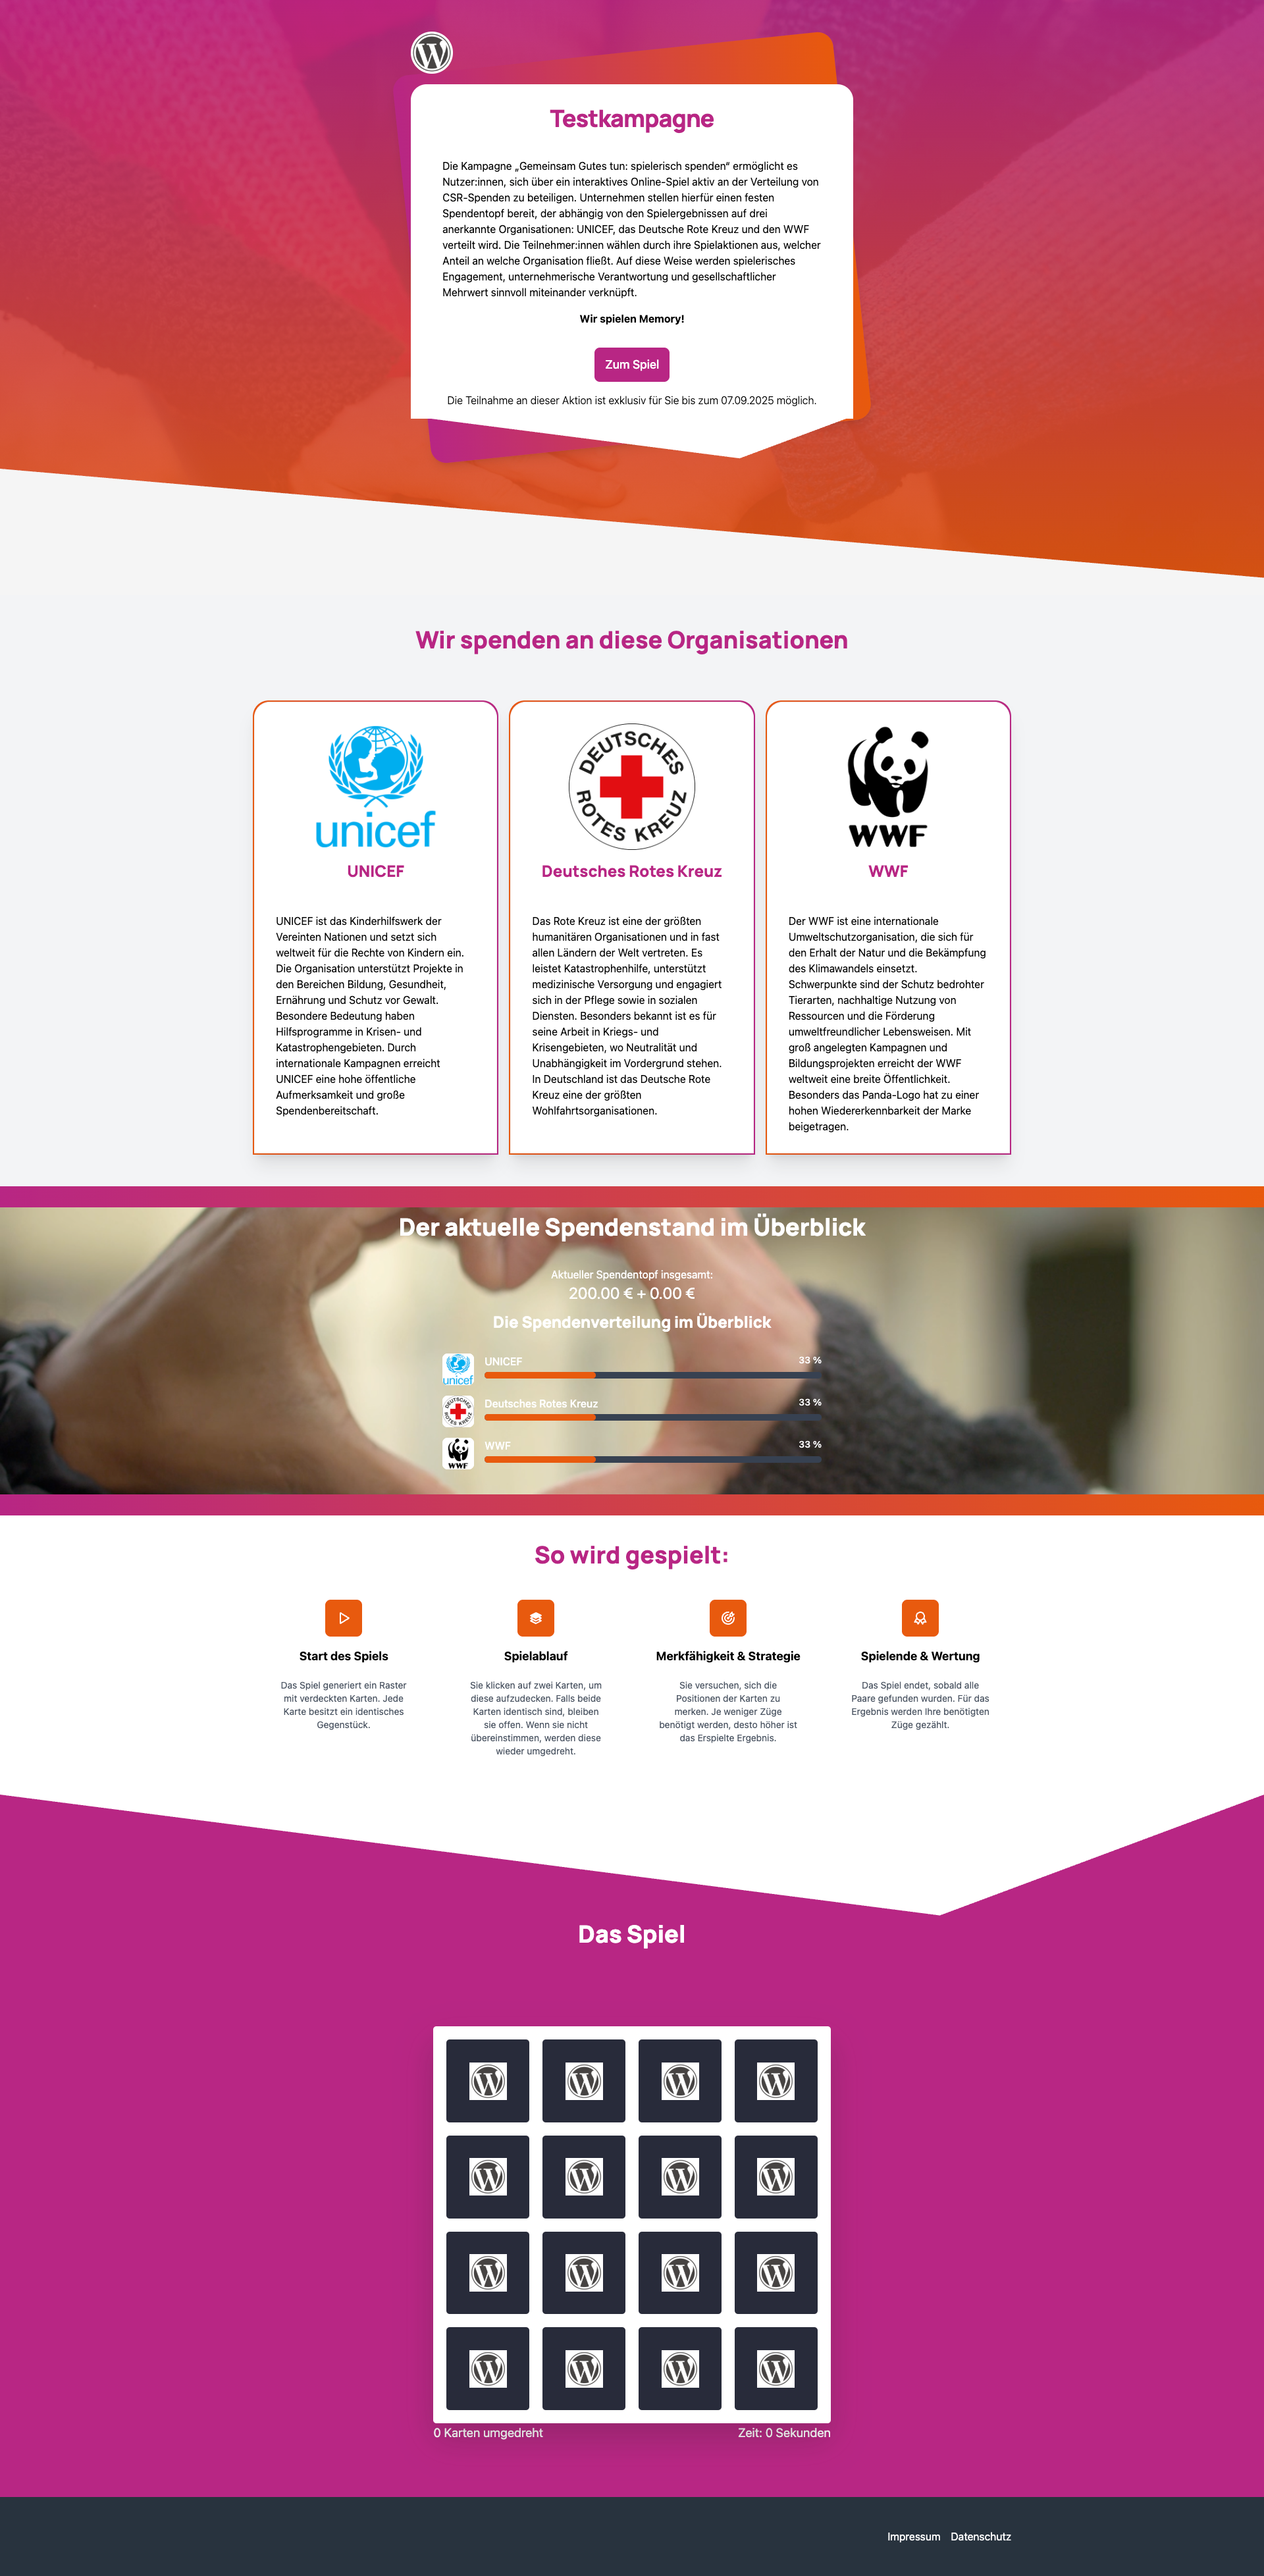
\includegraphics[width=0.66\textwidth]{images/legacy_landingpage_frontend}
    \caption{Gesamte Landingpage von Charigame im WordPress \\Frontend  (eigene Darstellung)}
    \label{fig:landing-frontend-legacy}
\end{figure}

\begin{figure}[H]
    \centering
    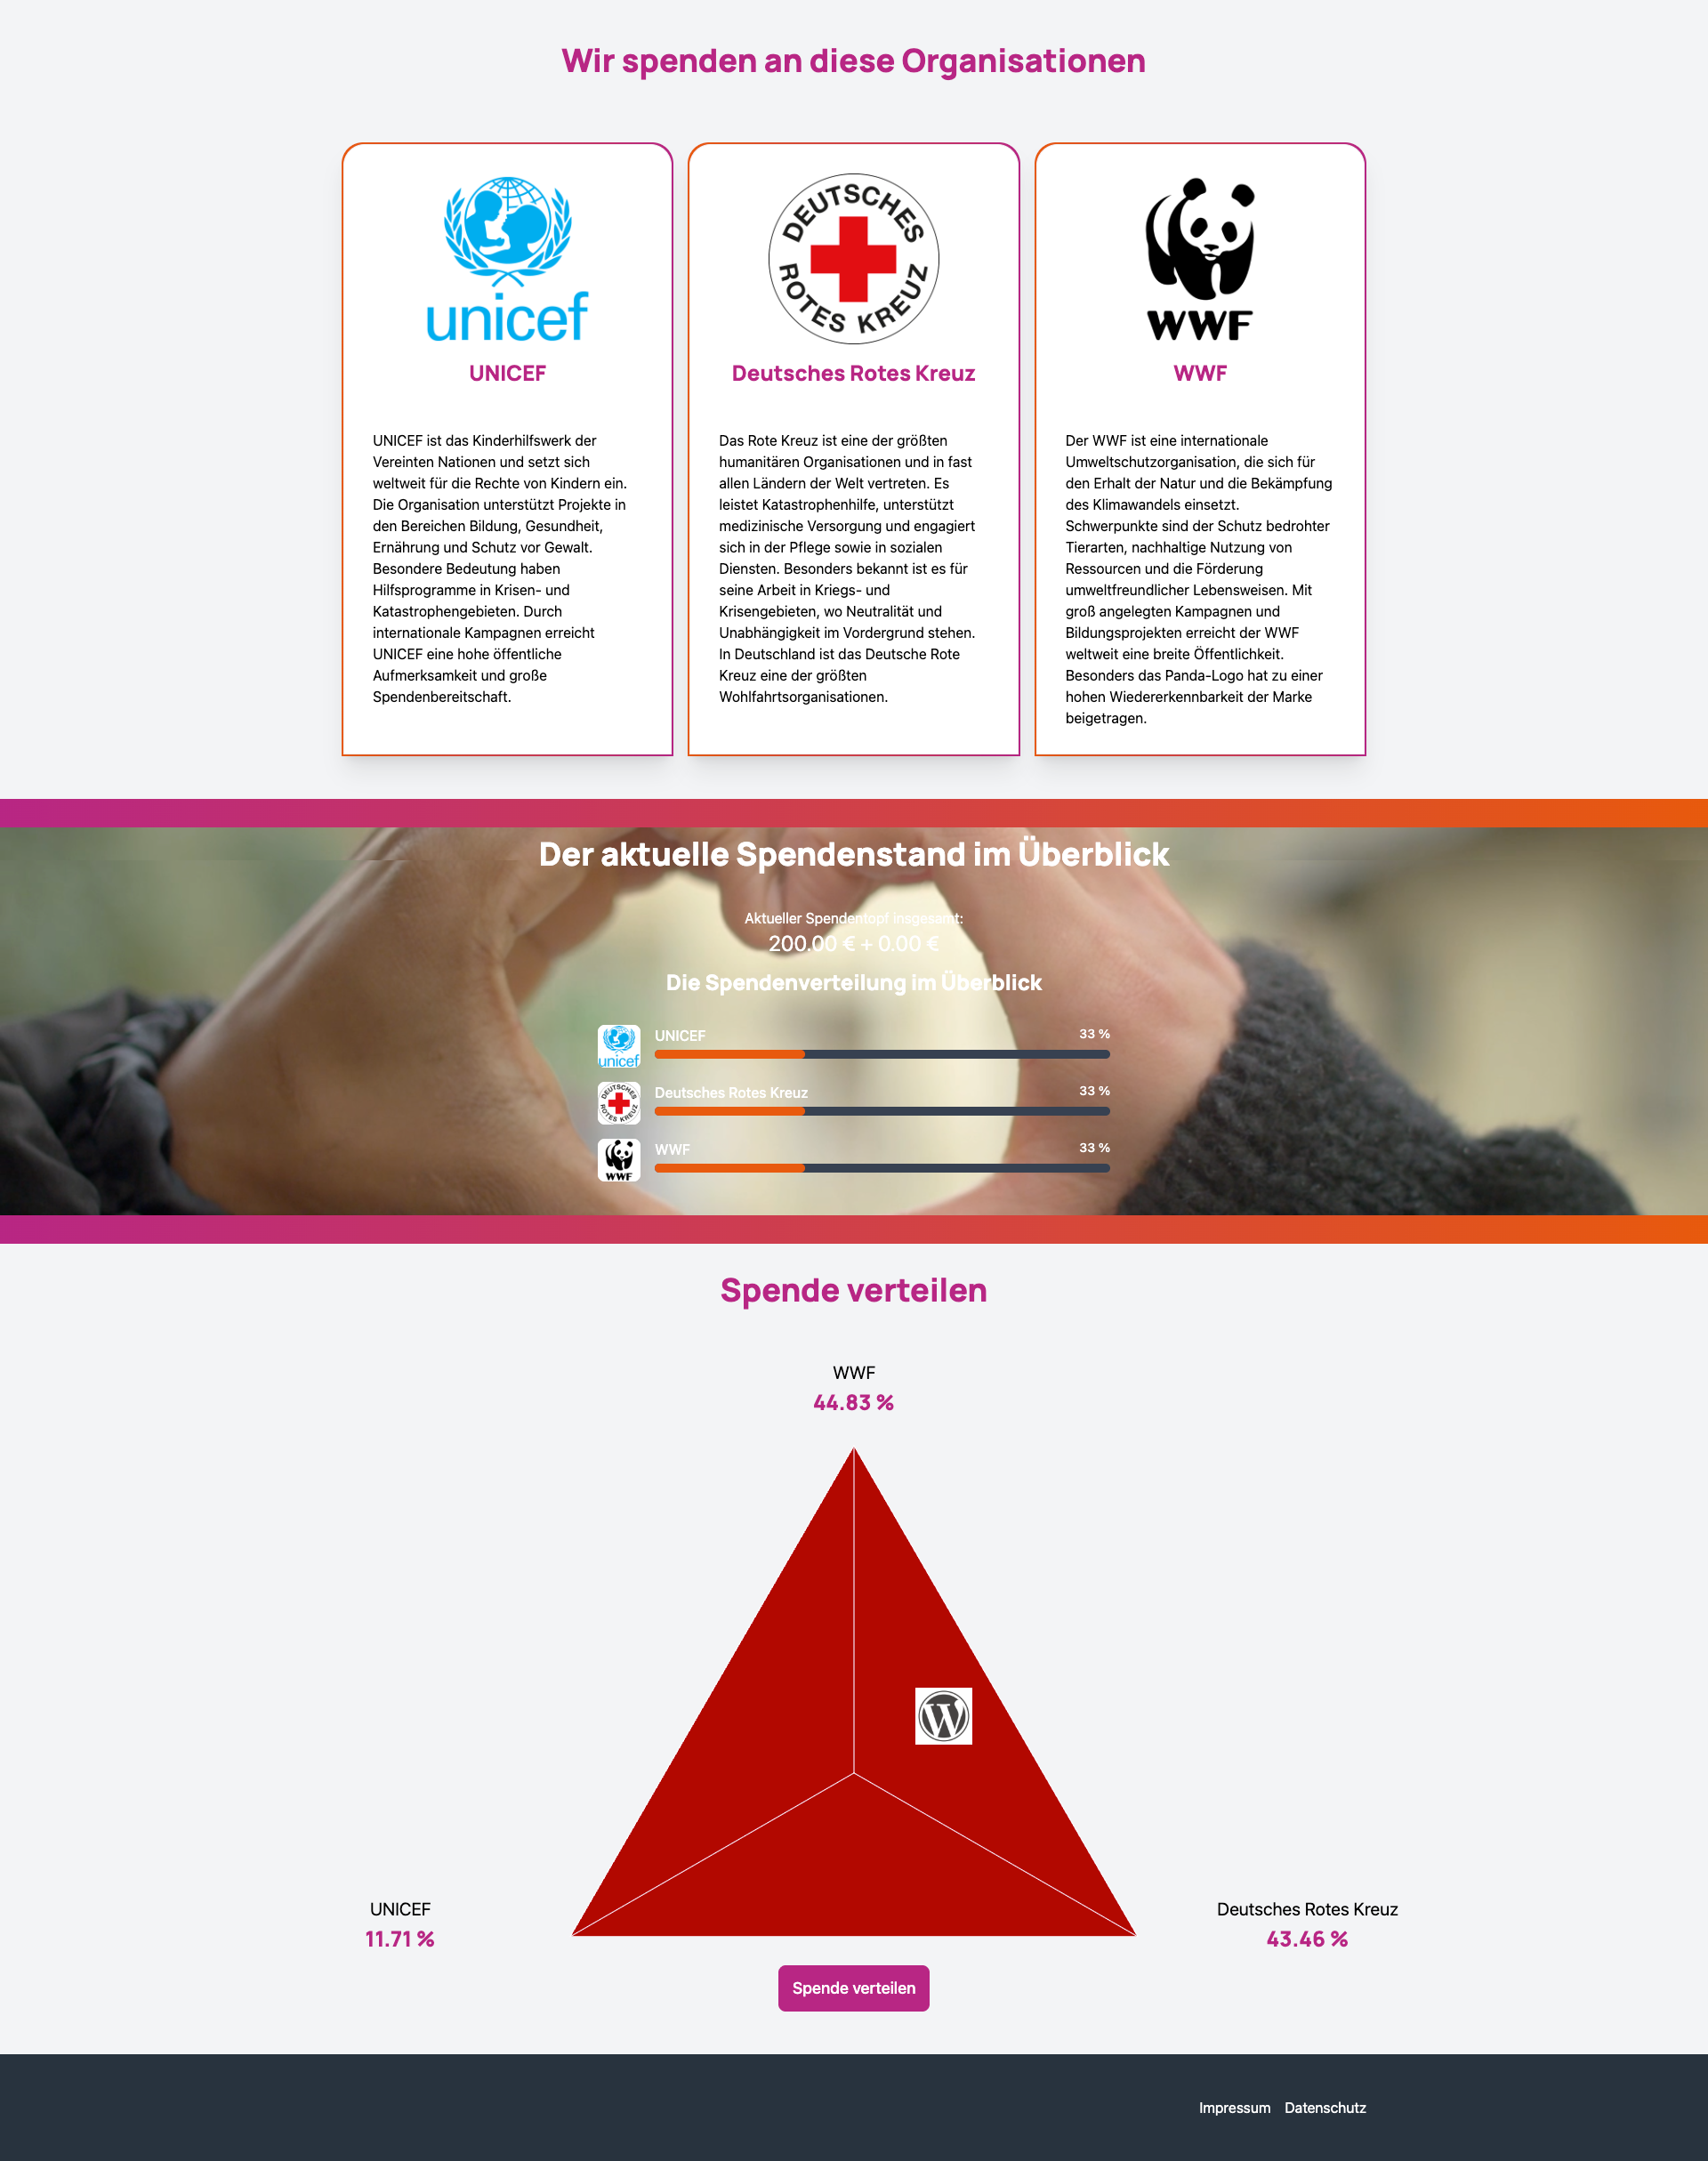
\includegraphics[width=1\textwidth]{images/legacy_verteilung_frontend}
    \caption{Spendenverteilungsseite von Charigame im WordPress Frontend (eigene Darstellung)}
    \label{fig:distribution-frontend-legacy}
\end{figure}

\begin{figure}[H]
    \centering
    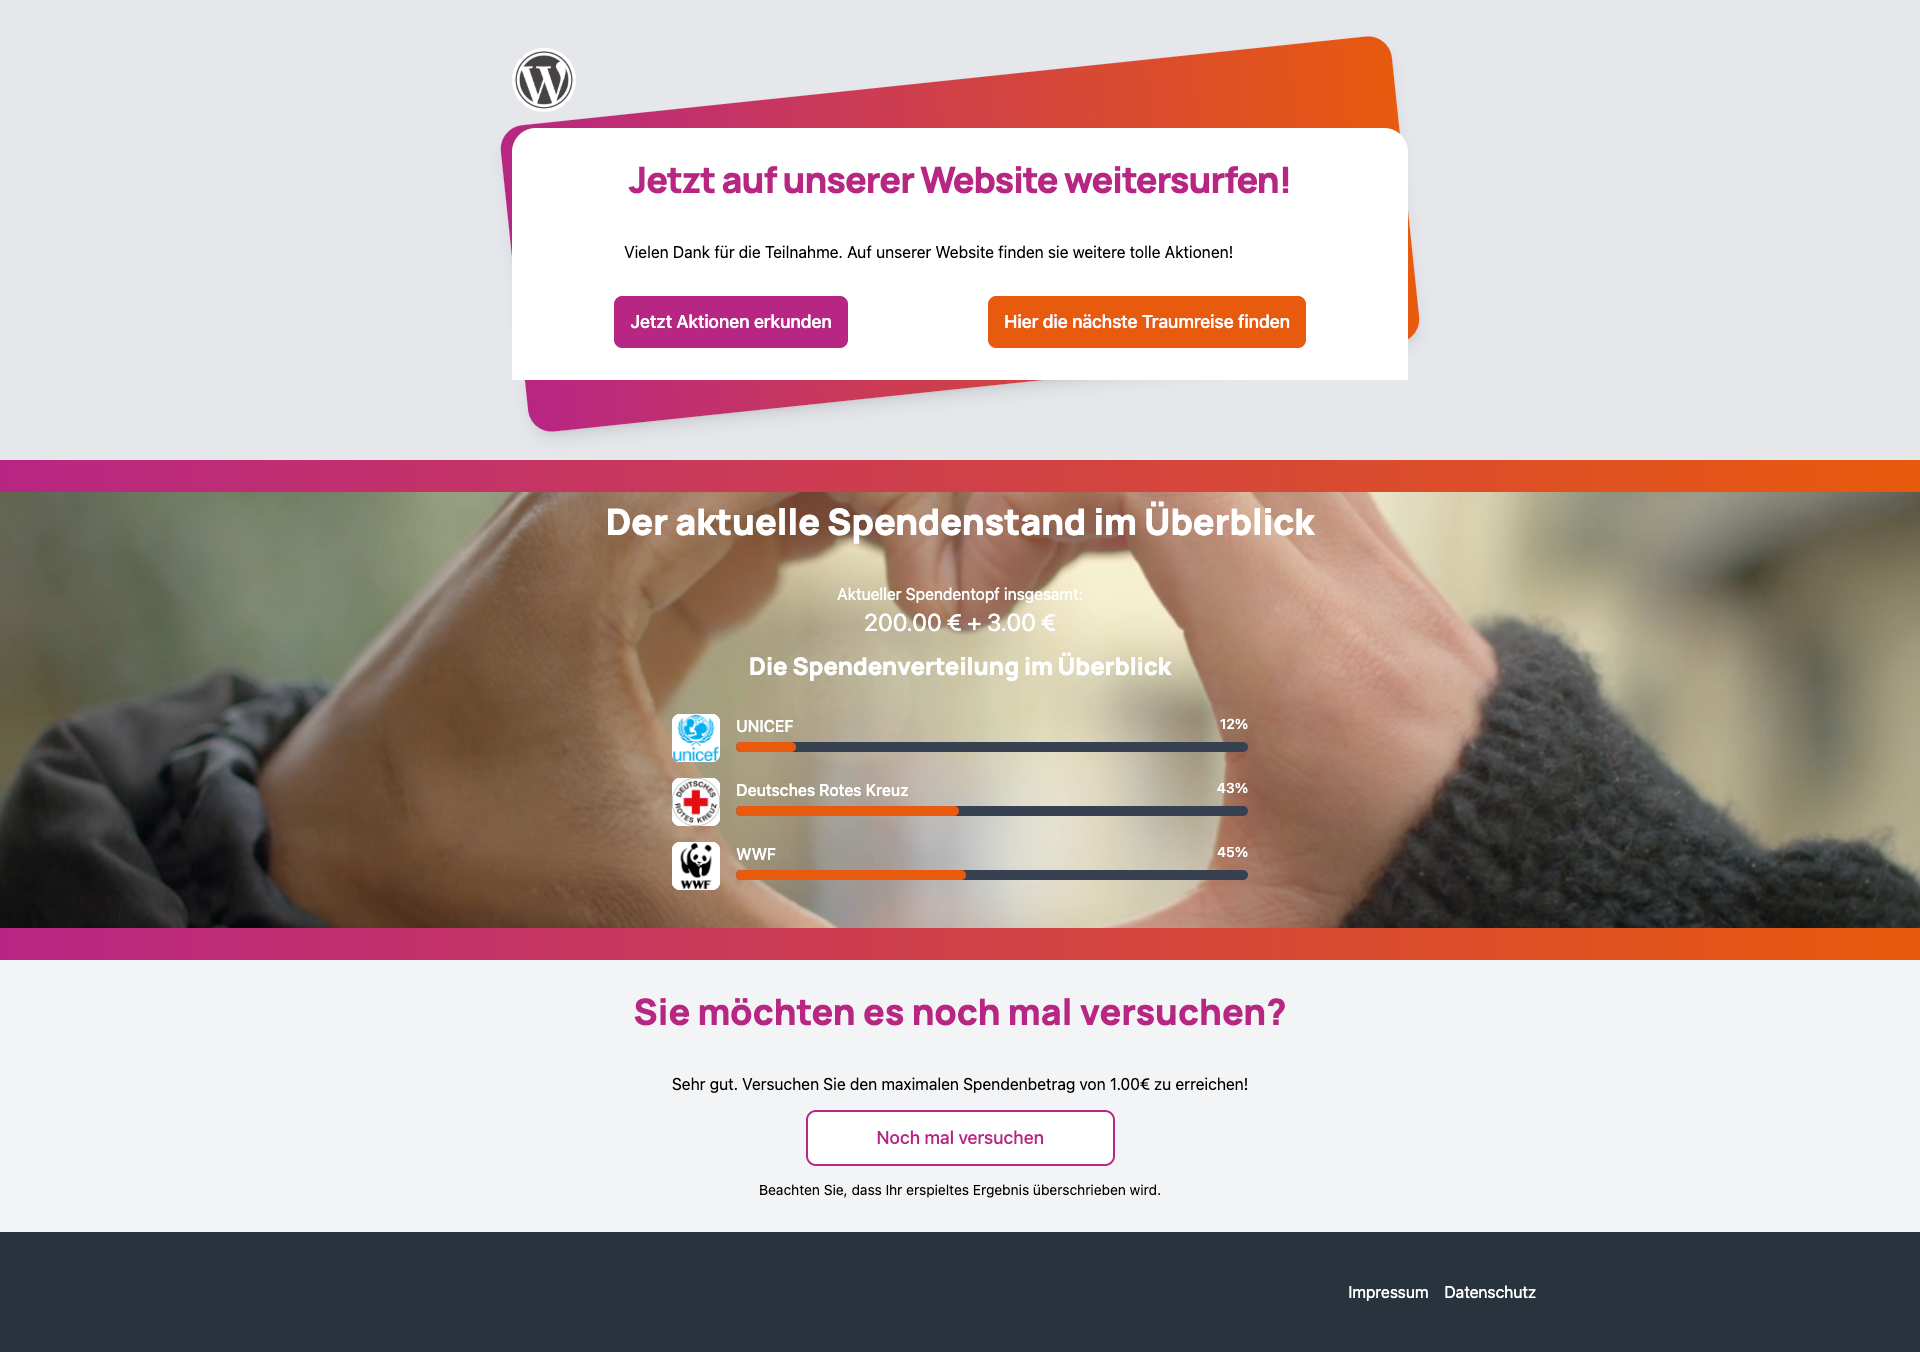
\includegraphics[width=1\textwidth]{images/legacy_dankesseite_frontend}
    \caption{Dankesseite von Charigame im WordPress Frontend (eigene Darstellung)}
    \label{fig:dankesseite-frontend-legacy}
\end{figure}

\KOMAoptions{open=any}
%
\chapter*{Erklärung}
%
Ich versichere, die von mir vorgelegte Arbeit selbstständig verfasst zu haben. Alle Stellen, die wörtlich oder sinngemäß aus veröffentlichten oder nicht veröffentlichten Arbeiten anderer oder der Verfasserin/des Verfassers selbst entnommen sind, habe ich als entnommen kenntlich gemacht. Sämtliche Quellen und Hilfsmittel, die ich für die Arbeit benutzt habe, sind angegeben. Die Arbeit hat mit gleichem Inhalt bzw.\ in wesentlichen Teilen noch keiner anderen Prüfungsbehörde vorgelegen.
\par
Anmerkung: In einigen Studiengängen findet sich die Erklärung unmittelbar hinter dem Deckblatt der Arbeit.
\\[3cm]
%
\begin{tabular}{@{}l@{}}%
\rule{0.35\textwidth}{0.4pt}\\
Ort, Datum%
\end{tabular}%
\hfill%
\begin{tabular}{@{}l@{}}%
\rule{0.45\textwidth}{0.4pt}\\
Unterschrift%
\end{tabular}%
%
%
\end{document}